\hypertarget{earlyexiting}{%
	\chapter{Edge Offloading with Early Exiting}\label{ch:edgeoffloading}}
\thispagestyle{fancy}

In this chapter we implement our inference scheme utilizing early exiting \gls{dnn}s. Our scheme is flexible in the sense it can be used in different edge-centric architectures and it is adaptive to enable service at more stringent latency requirements than currently proposed in literature using a best effort approach. Section \ref{sec:edge-aee} presents our offloading scheme. Section \ref{sec:edge-system-model} defines the system model. Section \ref{sec:edge-implementation} describes our implementation. Section \ref{sec:edge-results} present our results. Lastly section \ref{sec:edge-summary} summarizes our results.

\section{\acrfull{aee} for Time-Critical Applications} \label{sec:edge-aee}

We propose \acrfull{aee}, an optimistic inference scheme based on early exit \gls{dnn}. It is optimistic, in the sense, that it uses a best effort approach to maximize the reliability. The scheme does not terminate at any early exit, but instead terminates when a deadline has passed. Thus, the inference is run until time is out. The scheme allows to use increasingly confident predictions from the continuous inference process. Our scheme is flexible, as it can function for on-device, edge offloading or collaborative inference architectures. 

\begin{figure}
	\captionsetup[subfigure]{justification=centering}
	\centering
	\subfloat[Continuois predictions\label{fig:offloading-scheme-successful}]{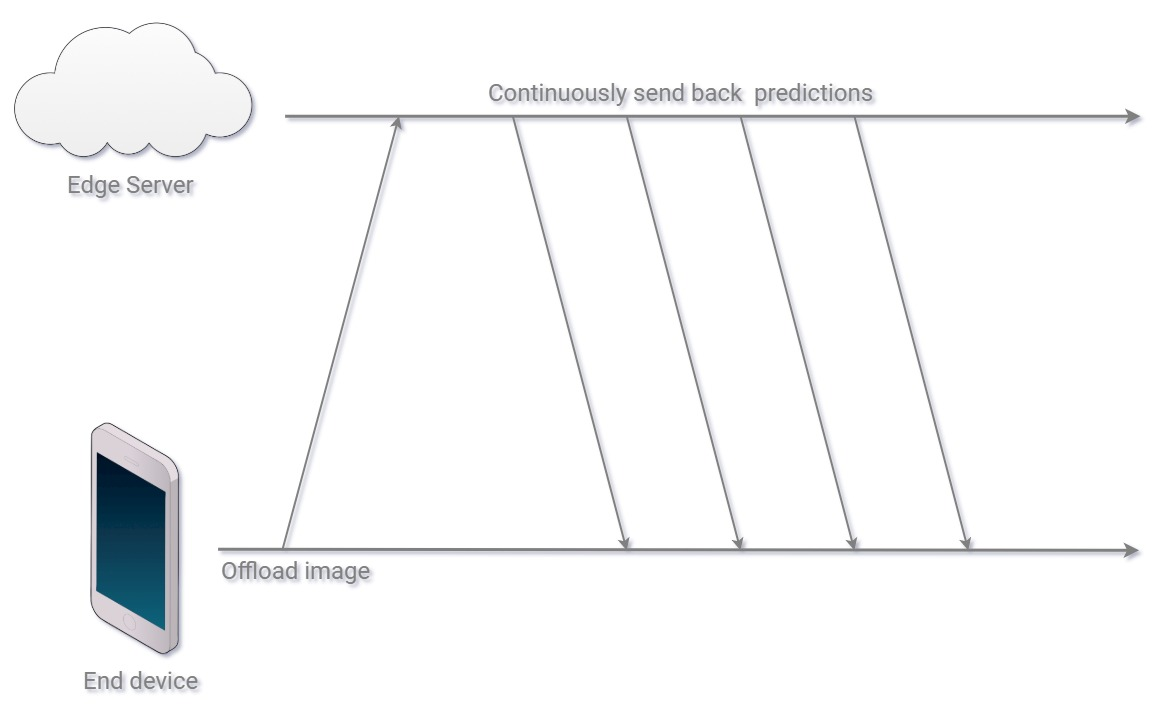
\includegraphics[width=.7\linewidth]{figures/models/timeline_all}}
\end{figure}
\begin{figure}
		\captionsetup[subfigure]{justification=centering}
	\centering
	\subfloat[Timeout of Continuois predictions\label{fig:offloading-scheme-timeout}]{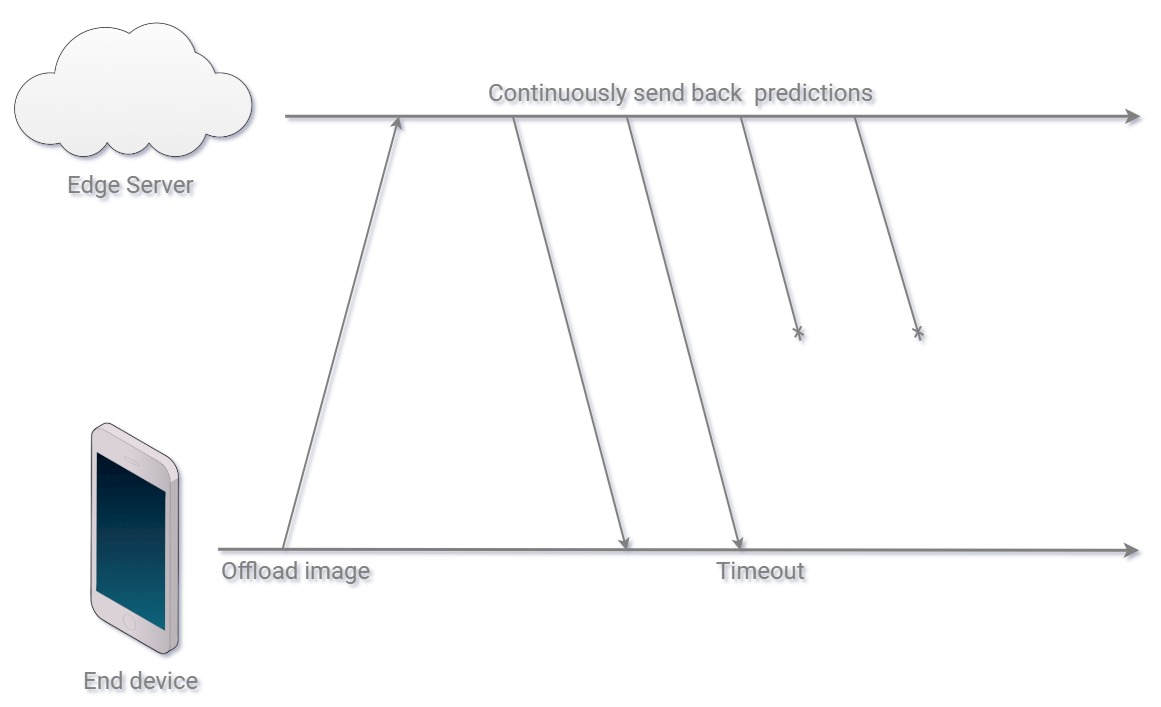
\includegraphics[width=.7\linewidth]{figures/models/timeline_timeout}}
	\caption[Offloading scheme]{\gls{aee} edge offloading: \protect\subref{fig:offloading-scheme-successful} continuous prediction received with no timeouts. \protect\subref{fig:offloading-scheme-timeout} 2 predictions received prior to timeout. }
	\label{fig:offloading-scheme}
\end{figure} 

In figure \ref{fig:offloading-scheme}, we present the scheme in the context of edge offloading. The data is immediately offloaded upon acquisition, from the end device to edge server, to not waste idle time on edge server. The edge server runs the inference process, and whenever a prediction is obtained from the early exit \gls{dnn} classifiers, it is sent back to the end device. Successively receiving prediction allow the user to select the most recent prediction from the deepest exit. Or alternatively, use information from all received predictions to select the most confident or use some combination function to select the best one. Figure \ref{fig:offloading-scheme-successful} illustrates the continuous reply of predictions. Figure \ref{fig:offloading-scheme-timeout} illustrates a case, where a timeout occurs and only two predictions are available 

\section{System Model} \label{sec:edge-system-model}

In this section we define the system model for \gls{aee}. Note the notations defined in chapter \ref{ch:earlyexit} is used here, i.e. $ C $ denotes the number of the image classes, $ N $ denotes the number of the exit points in a DNN, $ I $ denotes the number of images. 
		
	\begin{enumdescript}
		\item[Latency]  We use $ T_{i,n}^{cmp} $ to denote computation time irregardless of conventional inference model with a single exit, or early exit models with multiple. 
		
		We introduce two execution schemes, local processing and edge offloading.
		\begin{align}
		T_{i,n} = \begin{cases}
		T_{i,n}^{loc} \\
		T_{i,n}^{edge}
		\end{cases}
		\end{align}
		where $ T_{i,n}^{loc,cmp} $ denotes the computation time for local processing  and $ T_{i,n}^{edge,cmp} $ denotes computation time at the edge. 
		
		Due to the difference in computing resources, the computation time at edge is expected to be significantly lower than local computation time, i.e. $ T_{i,n}^{loc,cmp} > T_{i,n}^{edge,cmp} $. 
		
		Offloading for remote execution is only sensible, whenever time is saved compared to local execution, i.e.
		\begin{align*}
		T_{i,n}^{loc} > T_{i,n}^{edge}
		\end{align*}
		where the $ T_i^cmp,loc $ is calculated following eq. \ref{eq:t_ci-and-t_ee}.

		\begin{enumdescript}
			\item[Local Processing] Local runtime time is only defined by the time to compute the inference
			\begin{align}
			T_{i}^{loc}= T_{i}^{cmp,loc}
			\end{align}
			\item[Edge Offloading] Edge offloading runtime requires communication of data from local to remote and sending back results.
			\begin{align}
			T_{i}^{edge}=T_{i}^{com}+ T_{i}^{cmp,edge}
			\end{align}
			where $ T^{com}_i $ denotes the communication time, for both uplink time to transmit image $ i $ from local to edge, and downlink time of prediction reply from edge to local. The communication time $ T^{com}_i $ becomes an important factor for offloading decision, as the computing resources is expected to be more powerful on the edge, hence computing time is expected to be lower at the edge.
			

		\end{enumdescript}
	
		\item[Accuracy] The opportunities to receive multiple predictions within the time frame, may be able to improve the accuracy and reduce undesired overthinking, using the output results of the first $ n $ exit points to combine the information, to select the most confident class label $ \bm{\hat{c}}^f_i $. 
		\begin{align}
		\bar{A}^f &= 1 - \frac{1}{I} \sum_{i=1}^{I}\mathbb{I}\left(\left|\hat{c}_i^f-c_i\right|\right)
		\end{align}
		where the predicted class label $ \hat{c}_i^f = f(\bm{\hat{y}}_{i,1},\dots, \bm{\hat{y}}_{i,n}) $ is the output of a function, that combines the score vector output from the available exit predictions. 
	
		There are several ways to define combination function $ f\left(\bm{\hat{y}}_{i,1}, \dots, \bm{\hat{y}}_{i,n}\right) $
		\begin{enumdescript}
			
			\item[Latest Recieved Prediction] Under the assumption, that the last recieved prediction i.e. from deepest within the model has a better chance of being correct, as the exit has a higher accuracy than earlier exits. We define the method \emph{latest}, where we constrain ourselves to only use the most recent prediction $n$.
			\begin{align}
			f\left(\bm{\hat{y}}_{i,1}, \dots, \bm{\hat{y}}_{i,n} \right) = \hat{c}_{i,n}^{*}
			\end{align}
			
			\item[Max Confidence] This method uses the most confident prediction among all received exit predictions. It is used in \cite{kaya_shallow-deep_nodate}, which reports improvement on the \gls{cifar10}, \gls{cifar100} and \gls{tinyimagenet}. The measure is based on the assumption, that an exit obtaining a higher score is more confident, hence improving the accuracy.
			\begin{align}
			\begin{split}
			f\left(\bm{\hat{y}}_{i,1}, \cdots, \bm{\hat{y}}_{i,n} \right) =  \arg \underset{c}{\max} \{\hat{y}^*_{i,1}, ..., \hat{y}^*_{i,C} \},
			\\ \text{where\:} \hat{y}^*_{i,c} = \max \{\hat{y}_{i,1,c}, ..., \hat{y}_{i,n,c}\}
			\end{split}	
			\end{align}
			\item[Sum Confidence] The collective knowledge from all exits can be used by summing the scores by class from all received predictions. The class with the highest score becomes the prediction.
			\begin{align}
			\begin{split}
			f\left(\bm{\hat{y}}_{i,1}, \dots, \bm{\hat{y}}_{i,n} \right) = \arg \underset{c}{\max} \{s_{i,1}, \dots, s_{i,C}\}, \\ \text{where\:} s_{i,c} = \sum_{j=1}^{n}\hat{y}_{i,n,c}\: \forall \ 1\le c \le C
			\end{split}
			\end{align}
			
			%				\item[weighted sum confidence] this method perform a weighted sums of the respective class scores for all exit predictions and chooses the highest scoring class. 
			%
			%				\begin{align}
			%				\begin{split}
			%					f\left(\bm{\hat{y}}_{i,1}, \dots, \bm{\hat{y}}_{i,n} \right) = \arg \underset{n}{\max} \{s_{i,1}, \dots, s_{i,C}\},\\ \text{where\:} s_{i,n} = \sum_{j=1}^{n}w_n \hat{y}_{i,n,c} \text{\:for\:} \forall \ 1\le c \le C
			%				\end{split}	
			%				\end{align}
			
			\item[Max Score Margin] driven by the results in chapter \ref{ch:earlyexit}, the score-margin did show improvement as score threshold. The score margin from all received predictions is determined, and the largest value wins.
			\begin{align}
			\begin{split}
			f\left(\bm{\hat{y}}_{i,1}, \dots, \bm{\hat{y}}_{i,n} \right) =c^*_{1,\hat{n}},\\
			\text{where\:} \hat{n} \in \{1, 2, ..., n\}
			\end{split}	
			\end{align}
			this means $ \hat{n} $ is the exit, that provided the prediction with largest score margin, i.e.
			\begin{align*}
			\begin{split}
				\hat{n} = \arg \underset{j}{\max} \left\{f_{margin}(\bm{y}_{i,1}), ..., f_{margin}(\bm{y}_{i,n})\right\} ,\\
				\text{where\:} j \text{\:is an integer and\:} 1 \le j \le n
			\end{split}
			\end{align*}
			Note, $ f_{margin} $ is defined in eq. \ref{eq:f_margin}.
		\end{enumdescript}
	
		\item[Reliability]  We still define the reliability as in chapter \ref{ch:earlyexit}, as the fraction of samples, that can be correctly classified given a latency threshold $ \delta $.
		
		\begin{align}
		R^f= \bar{A^f} \cdot (1-\overline{F}^{to})
		\end{align}
		
		The timeout probability $ \overline{F}^{to} $ is also still defined as the number of samples not able to meet the delay requirement out of all samples in the set. However, our latency is now not only dependent on computation time, but also communication time when offloading.
		\begin{align}
		\overline{F}^{to}=\frac{1}{I}\sum_{i=1}^{I} \mathbb{I}\left(T_{i,n}-\delta\right)
		\end{align}
		and as before
		\begin{align*}
			T_{i} = \begin{cases}
				T_{i}^{loc} \\
				T_{i}^{edge}
			\end{cases}
		\end{align*}
		We have a delay violation, if no prediction is provided before the deadline, i.e. $ T_{i} > \delta $  
	
		\item[Problem] As in chapter \ref{ch:earlyexit}, we define a maximization problem. The aim is to maximize the reliability for each image by selecting the best possible exit
		\begin{maxi}
			{\bm{n}}{\bar{R}^f}
			{}{}
			%\addConstraint{T_{i,n}}{\leq \delta}
		\end{maxi}
		where $ \bm{n} = \left\{ n_1, n_2, \dots, n_I \right\}$ is a vector to denote which exit point would be used for prediction image $ i $ for available exit point $ n_i \in \left\{1,2, \dots, N\right\} $.
		
		Similar to chapter \ref{ch:earlyexit}, we solve this problem with the best effort scheme, i.e., feed each exit results back and let user decide the prediction. Instead of upfront exit decision. For three reasons:
		\begin{enumerate}
			\item latency uncertainty, not least from newly introduced communication, makes it hard to make an exit decision in advance
			\item avoid overhead from algorithm to make decision
			\item the classifier of each exit point does not add a significant overhead
		\end{enumerate}
		
			
	\end{enumdescript}  

\section{Implementation} \label{sec:edge-implementation}

The offloading scheme is implemented as a client/server application \cite{sommerville_software_2015}, illustrated by the sequence diagram in figure \ref{fig:sequence-diagram}. 

\begin{figure}
	\captionsetup[subfigure]{justification=centering}
	\centering
	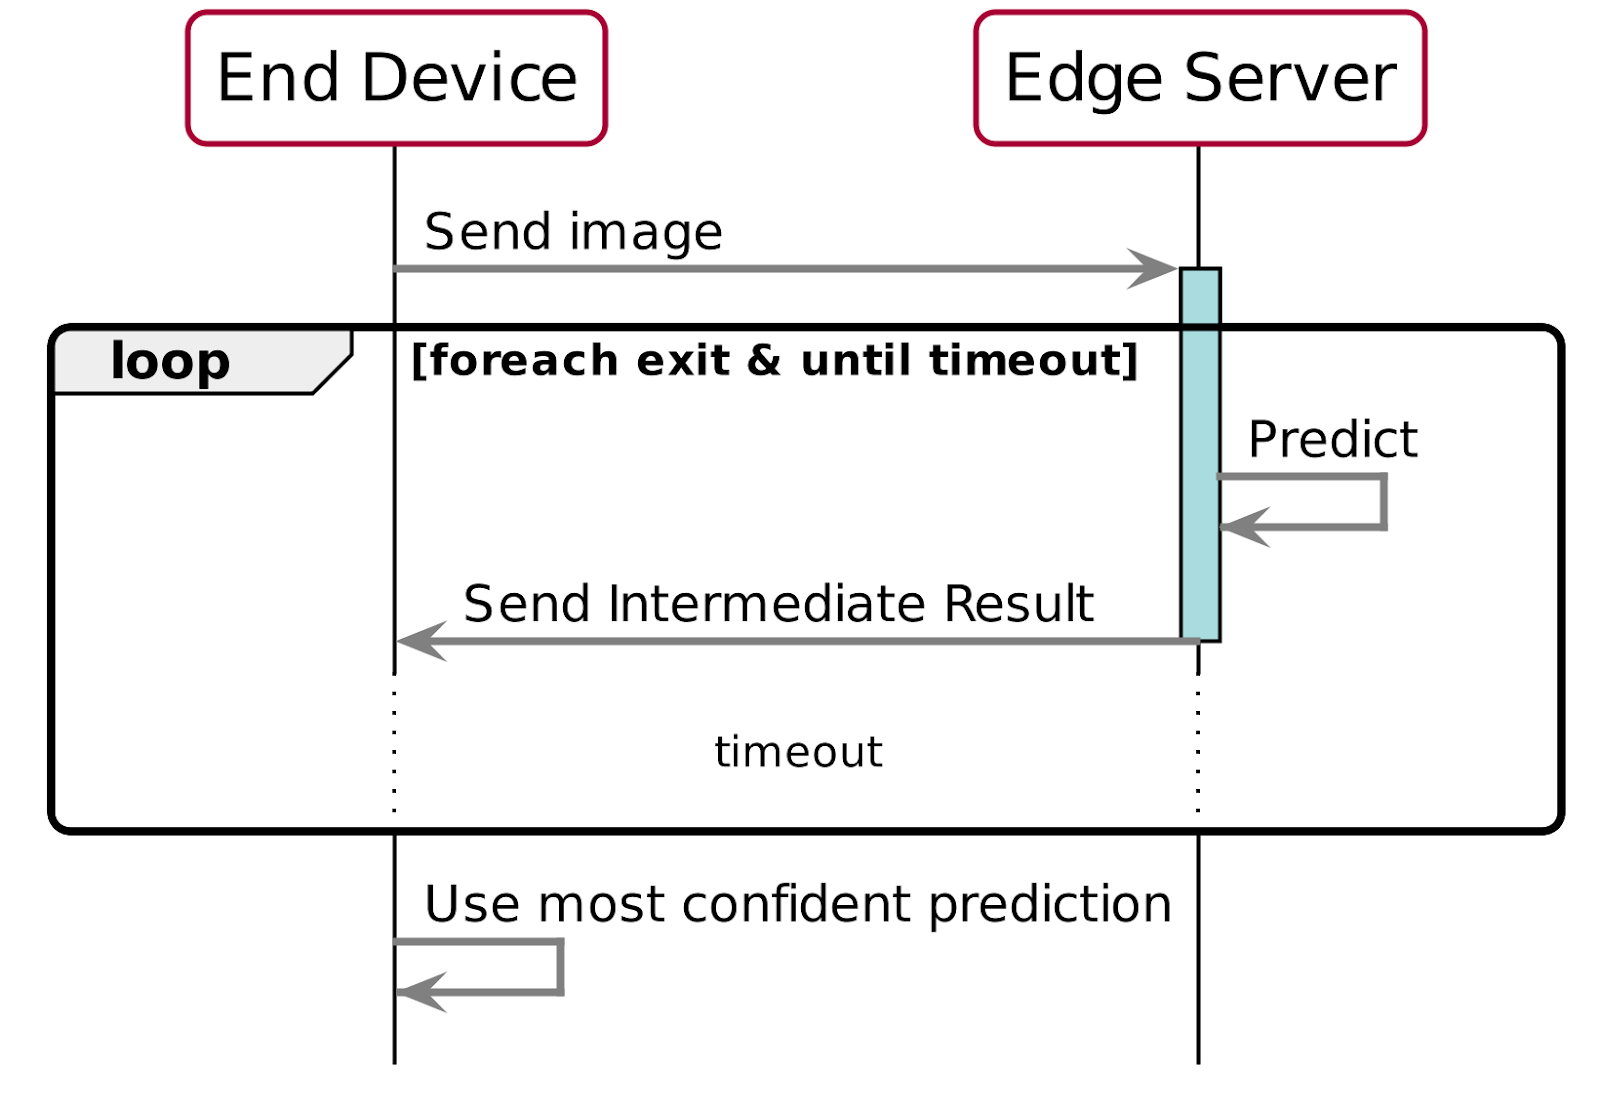
\includegraphics[width=.7\linewidth]{figures/models/sequence_diagram}
	\caption[Sequence Diagram \acrshort{aee}]{Sequence Diagram \acrshort{aee}: The client and server establishes a TCP socket connection. The client loads a samples from the \gls{min100} validation set, and streams the sample to the server. The server preprocess the sample and runs the model inference. As soon as, prediction are obtained, a thread is spawned, to stream the results back to the end device. }
	\label{fig:sequence-diagram}
\end{figure}

The implementation is written in \gls{python} using the \gls{python} Socket API \cite{noauthor_socket_nodate}, \gls{pytorch} \cite{paszke_automatic_2017} and \gls{torchvision} \cite{marcel_torchvision_2010}. The client is deployed on the \gls{nuc} and the server on \gls{jetson} and \gls{gpu-ws}. The servers are LAN connected to the router and the client is connected over the WLAN.

\paragraph{Information Combination}

We send back the top-5 predictions to allow information combination and reduce the data size of the reply. We use top-5, since the correct class is within these 5 predictions close to 90 \% of the time having just two predictions available for any of the models, see figure \ref{fig:top-5-cumulative}.

To combine top-5 prediction information from $ n $ exits, we must expand the vectors back to the original class space of $ C $ dimensions.

Each exit outputs two 5-dimensional vectors. $\bm{\hat{c}}_{i,k}^{top5}$ contains the labels of the top-5 predictions and $ \bm{\hat{y}}_{i,k}^{top5}$ contain the class scores of the top-5 predictions. 

\begin{align}
\begin{split}
\bm{\hat{c}}_{i,n}^{top5} &= \begin{bmatrix}
\hat{c}_{i,n}^{1st} & \phantom{.}\hat{c}_{i,n}^{2nd} & \phantom{.}\hat{c}_{i,n}^{3rd} & \phantom{.}\hat{c}_{i,n}^{4th} & \phantom{.}\hat{c}_{i,n}^{5th}
\end{bmatrix}, \\
\bm{\hat{y}}^{top5}_{i,n} &= \begin{bmatrix}
\hat{y}_{i,n}^{1st} & \phantom{.}\hat{y}_{i,n}^{2nd} & \phantom{.}\hat{y}_{i,n}^{3rd} & \hat{y}_{i,n}^{4th} & \phantom{.}\hat{y}_{i,n}^{5th}
\end{bmatrix}
\end{split}
\end{align}

The vectors are sorted from highest to lowest, hence the score $ \hat{y}_{i,k}^{1st} $ is associated the class label $ c_{i,k}^{1st} $ etc. 

We define an expansion function, which takes the top-5 score vector $ \bm{\hat{y}}_{i,n}^{top5}$ and top-5 class label vector  $\bm{\hat{c}}_{i,n}^{top5}$ as input  $ f_{expand}\left(\bm{\hat{y}}_{i,n}^{top5},\bm{\hat{c}}_{i,n}^{top5}\right) $ and outputs a $ C $-dimensional score vector, with the scores at corresponding class index of the label vector, with the remaining indices are zero.
\begin{align}
f_{expand}\left(\bm{\hat{y}}_{i,n}^{top5},\bm{\hat{c}}_{i,n}^{top5}\right) = 
\begin{bmatrix}
\hat{y}_{i,n,1} & \hat{y}_{i,n,2} & \hat{y}_{i,n,c} & \dots & \hat{y}_{i,n,C}
\end{bmatrix}_{1 \times C}
\end{align}


\subparagraph{Example: Expansion of a 10 class problem} 
\blockquote[]{	 	
	For this $C=10$ example, we receive two output vectors $\bm{\hat{c}}_{i,n}^{top5}$ and $ \bm{\hat{y}}_{i,n}^{top5}$.
	\begin{align*}
	\bm{\hat{c}}_{i,n}^{top5} &= \begin{bmatrix}
	\phantom{0}0\phantom{.0} & \phantom{0}3\phantom{.0} & \phantom{0}6\phantom{.0} & \phantom{0}8\phantom{.0} & \phantom{0}9\phantom{.0}
	\end{bmatrix},\\
	\bm{\hat{y}}_{i,n}^{top5} &= \begin{bmatrix}
	0.80 & 0.10 & 0.05 & 0.03 & 0.01
	\end{bmatrix}
	\end{align*}
	We use our expansion function $ f_{expand}\left(\bm{\hat{y}}_{i,n}^{top5},\bm{\hat{c}}_{i,n}^{top5}\right) $, which return the score vector $ \mathbf{\hat{y}}_{i,n}$, for the respective classes in $ \bm{c}_{i,n} $
	\begin{align*}
	\mathbf{\hat{y}}_{i,n}  &= \begin{bmatrix}
	0.80 & 0.00 & 0.00 & 0.10 & 0.00 & 0.00 & 0.05 & 0.00 & 0.03 & 0.01
	\end{bmatrix}_{1 \times 10} \\
	\bm{c}_{i,n} &= \begin{bmatrix}
	\phantom{0}0\phantom{.0} & \phantom{0}1\phantom{.0} & \phantom{0}2\phantom{.0} & \phantom{0}3\phantom{.0} & \phantom{0}4\phantom{.0} & \phantom{0}5\phantom{.0} & \phantom{0}6\phantom{.0} & \phantom{0}7\phantom{.0} & \phantom{0}8\phantom{.0} & \phantom{0}9\phantom{.0}
	\end{bmatrix}_{1 \times 10},
	\end{align*}
}      

Having multiple score vectors $ \left\{\bm{\hat{y}}_{i,1}, \dots, \bm{\hat{y}}_{i,n}\right\}  $ in the original class space, allow us to formulate a $ n \times C $ score matrix $ \bm{\hat{Y}}_{i}^{n \times C} $.
\begin{align}
	\bm{\hat{Y}}_{i}^{n \times C} =
	\begin{bmatrix}
		\hat{y}_{i,1,1} & \hat{y}_{i,1,2} & \dots & \hat{y}_{i,1,C} \\
		\hat{y}_{i,2,1} & \hat{y}_{i,,2} & \dots & \hat{y}_{i,2,C} \\
		\vdots & \vdots & \ddots & \vdots \\
		\hat{y}_{i,n,1} & \hat{y}_{i,n,2} & \dots & \hat{y}_{i,n,C}
	\end{bmatrix}
\end{align}

Formulating as matrix ease the implementation of combination functions using \gls{numpy} \cite{oliphant_numpy:_2006}, to use methods from linear algebra, e.g. finding the maximum entry and summing the columns.
\subparagraph{Example: Prediction matrix and information combination} 
\blockquote[]{	 	
	For this classification example, the number of classes $C=10$. Within a time frame we receive predictions from 3 exits. We assume the predictions have been expanded.
	\begin{align*}
	\bm{c}_{i} &= \begin{bmatrix}
	\phantom{0}0\phantom{.0} & \phantom{0}1\phantom{.0} & \phantom{0}2\phantom{.0} & \phantom{0}3\phantom{.0} & \phantom{0}4\phantom{.0} & \phantom{0}5\phantom{.0} & \phantom{0}6\phantom{.0} & \phantom{0}7\phantom{.0} & \phantom{0}8\phantom{.0} & \phantom{0}9\phantom{.0}
	\end{bmatrix}_{1 \times 10},\\
	\bm{\hat{y}}_{i,1}  &= \begin{bmatrix}
		0.80 & 0.00 & 0.00 & 0.10 & 0.00 & 0.00 & 0.05 & 0.00 & 0.03 & 0.01
	\end{bmatrix}_{1 \times 10}
	\\
	\bm{\hat{y}}_{i,2}  &= \begin{bmatrix}
		0.10 & 0.00 & 0.00 & 0.01 & 0.00 & 0.85 & 0.00 & 0.02 & 0.00 & 0.02
	\end{bmatrix}_{1 \times 10}
		\\
	\bm{\hat{y}}_{i,3}  &= \begin{bmatrix}
		0.15 & 0.00 & 0.00 & 0.02 & 0.01 & 0.00 & 0.00 & 0.80 & 0.00 & 0.02
	\end{bmatrix}_{1 \times 10}
	\end{align*}
	We construct the matrix $ \bm{\hat{Y}}_{i}^{n \times C} $
	\begin{align*}
			\bm{\hat{Y}}_{i}^{n \times C} =
		\begin{bmatrix}
		0.80 & 0.00 & 0.00 & 0.10 & 0.00 & 0.00 & 0.05 & 0.00 & 0.03 & 0.01 \\
		0.10 & 0.00 & 0.00 & 0.01 & 0.00 & 0.85 & 0.00 & 0.02 & 0.00 & 0.02 \\
		0.15 & 0.00 & 0.00 & 0.02 & 0.01 & 0.00 & 0.00 & 0.80 & 0.00 & 0.02 
		\end{bmatrix}_{3 \times 10}
	\end{align*}
	Using the defined combination functions, yield the following results:
	\begin{enumerate}
		\item Using the latest exit prediction the resulting prediction $  \hat{c}^{**}_{i} = \hat{c}^*_{i,3} = 7$.
		\item 	Using the maximum confidence the resulting prediction becomes $ \hat{c}^{**}_{i} =  5$ from exit 2.
		\item 	Using sum confidence we sum all columns to create a new score vector
		\begin{align*}
		\bm{\hat{y}^{**}_{i}} = 
		\begin{bmatrix}
		1.05 & 0.00 & 0.00 & 0.13 & 0.01 & 0.85 & 0.05 & 0.82 & 0.03 & 0.05
		\end{bmatrix}_{1 \times 10}
		\end{align*}
		Thus the resulting prediction becomes $ \hat{c}^{**}_{i} = 0$
		\item Using the score-margin we find the largest difference between the two highest scores in the 2nd row i.e. the second exit. $ f_{margin}\left(\bm{\hat{y}_{i,2}}\right) = \hat{y}_{i,2,5} - \hat{y}_{i,2,0} = 0.85 - 0.10 =0.75 $ Thus the resulting prediction becomes $ \hat{c}^{**}_i = 5$
	\end{enumerate}
	Evidently, combining the scores gives different outcomes in this theoretical yet realistic example.
	
}

\section{Results} \label{sec:edge-results}

In this section we present an analysis, that spawned the idea of combining prediction scores from multiple exits. We present the results using the different combination functions, and conclude that simply using the latest prediction is the better option. Furthermore we have made practical experiments offloading the inference task to the edge using both early exit and conventional models. We evaluate the impact of communication when offloading and compares local processing on the \gls{nuc} with offloading to either \gls{jetson} or \gls{gpu-ws}.

\subsection{Information Combination Analysis}

We want to examine the possibility to combine predictions from multiple exits to obtain a higher accuracy. A study of top-1 predictions results from all exits, revealed that, we too encounter overthinking as in \cite{kaya_shallow-deep_nodate}. In some cases an early exit correctly predicts a sample, which a later exit makes wrong. An example is the 6th sample from the \gls{bresnet}, $ c_6 $ is the ground truth class label, $ \bm{\hat{c}}_6 $ is the predicted class labels, $ \hat{y}^*_6 $ is the corresponding prediction score for the class label at all exits. $ b $ denotes the correctness of each exit as a binary value, where 1 is correct 0 is incorrect.
\begin{align*}
c_6=0,
\bm{\hat{c}}_{6}=
\begin{bmatrix}
0 \\
54 \\
62 \\
62
\end{bmatrix},
\bm{\hat{y}}^{*}_{6}=
\begin{bmatrix}
0.56 \\
0.32 \\
0.52 \\
0.62
\end{bmatrix} \text{\:and\:}
\bm{b}_{6}=
\begin{bmatrix}
1 \\
0 \\
0 \\
0
\end{bmatrix}
\end{align*}
Based on the scores the model is more confident about the last exit prediction, even though the prediction from the first exit is correct. Given the four entries of top-1 prediction, both latest or confidence max will output label 62. Analyzing the exit score have shown, that the score of a later exit is not always higher than the earlier exits, see figure \ref{fig:exit-highscore}.

\begin{figure}
	\captionsetup[subfigure]{justification=centering}
	\centering
	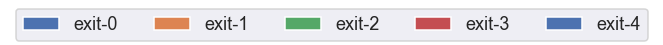
\includegraphics[width=.7\linewidth]{figures/edge/exit0-4_legend}
	\subfloat[B-ResNet]{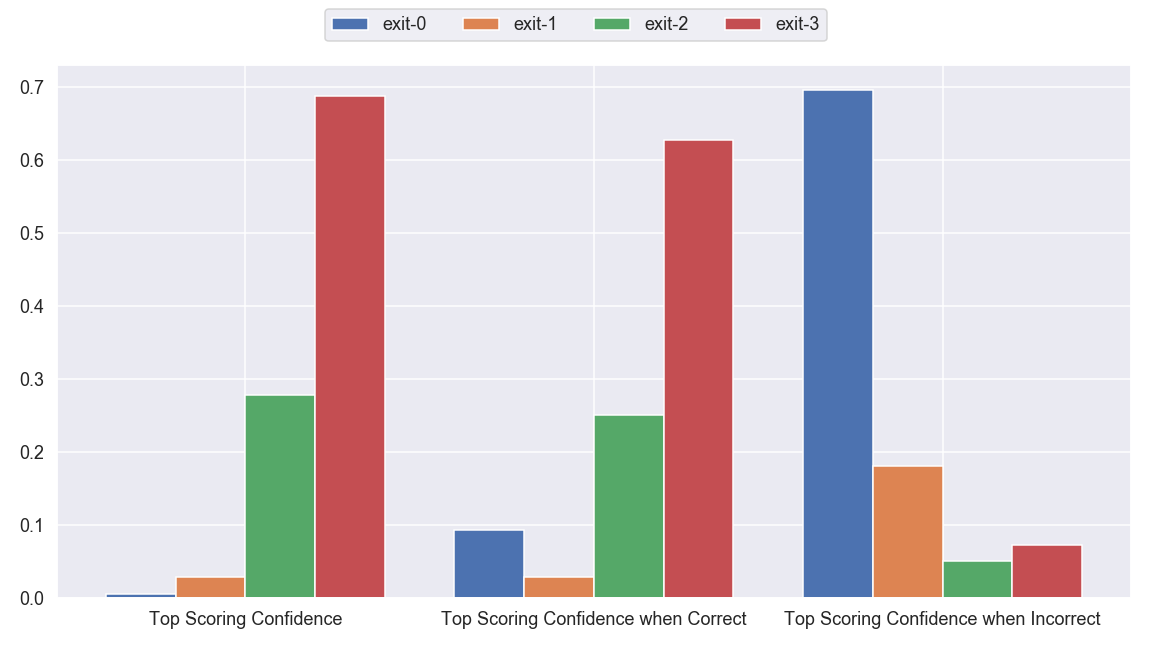
\includegraphics[width=.33\linewidth]{figures/edge/b-resnet_correctness}}
	\hfill
	\subfloat[B-DenseNet]{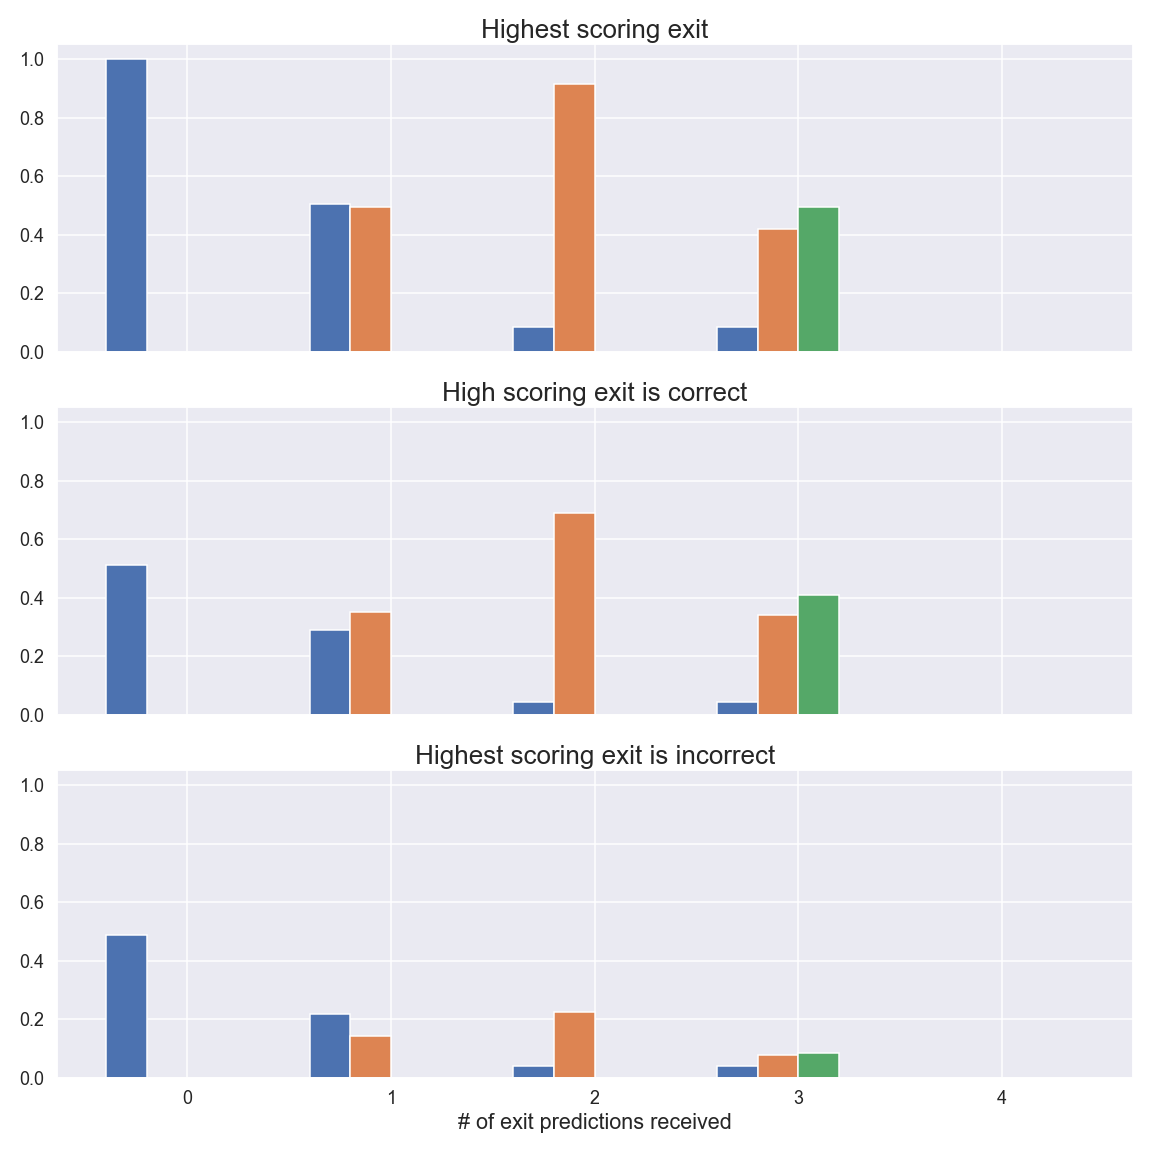
\includegraphics[width=.33\linewidth]{figures/edge/b-densenet_correctness}}
	\hfill
	\subfloat[MSDNet]{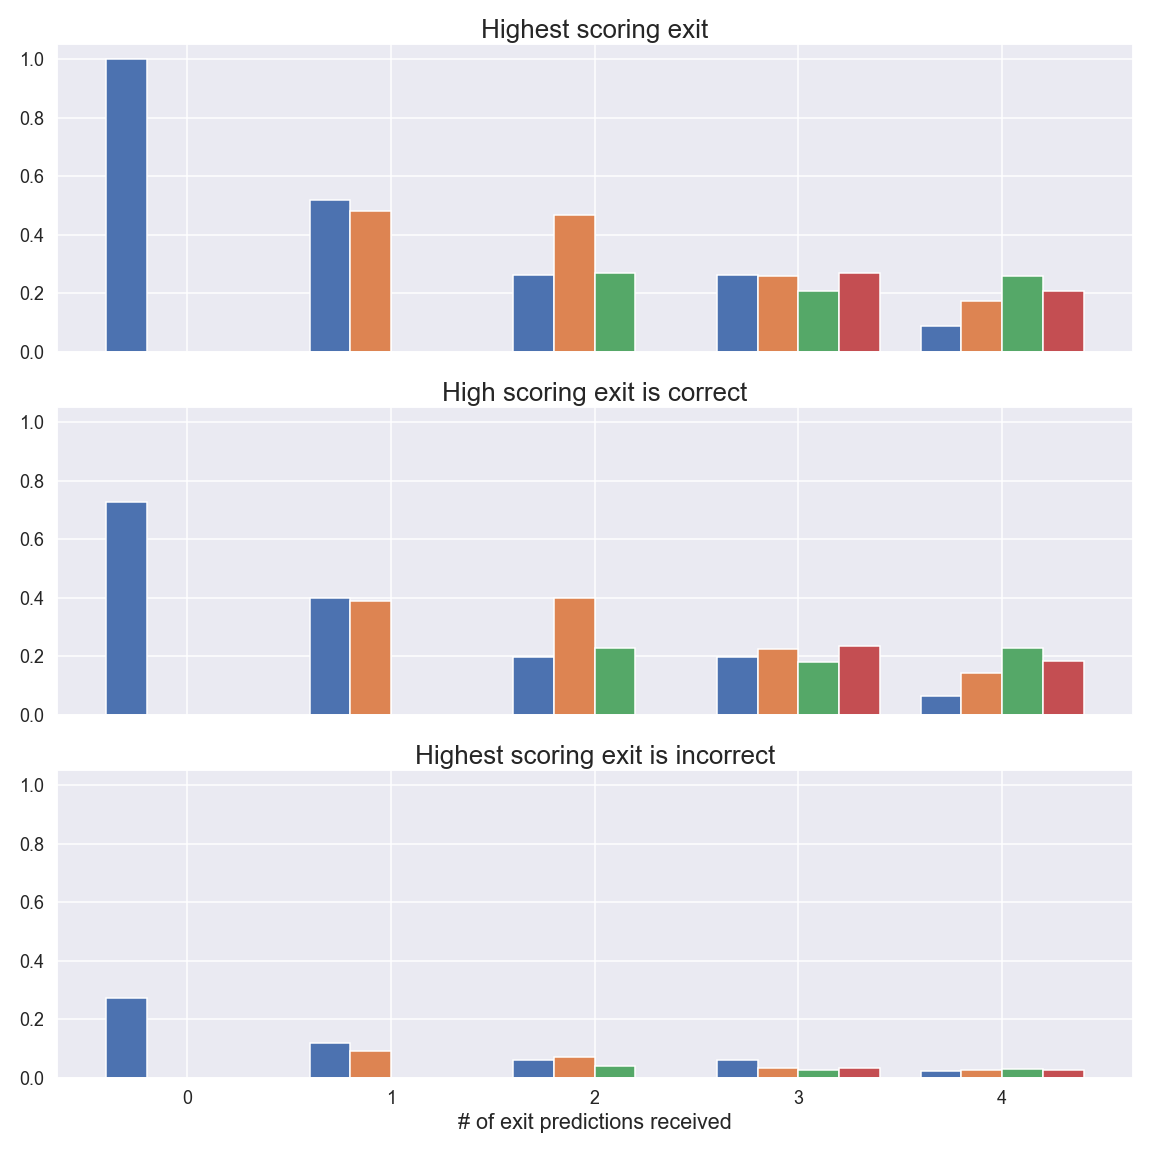
\includegraphics[width=.33\linewidth]{figures/edge/msdnet_correctness}}
	\caption[Model Highest Scoring Exit]{Model Highest Scoring Exit}
	\label{fig:exit-highscore}
\end{figure}

In fact, using the maximum score, as proposed in \cite{kaya_shallow-deep_nodate}, actually reduces the accuracy of the model, see table \ref{tbl:latest-vs-max}. It seems, that although the early exits achieve a higher score, they also introduces more uncertainty.  

\begin{minipage}[t]{\linewidth}
\begin{longtabu}{>{\bfseries}X|X|X}
	\caption[]{} \label{tbl:latest-vs-max} \\
	\toprule
	\rowfont{\bfseries}
	Model & Latest Received Prediction & Max Score   \tabularnewline
	\bottomrule
	\endfirsthead
	\multicolumn{3}{@{}l}{\textbf{\textcolor{black}{Table \ref{}:}} continued}\\
	\toprule
	\rowfont{\bfseries}
	Model & $Exit_N$ & max score    \tabularnewline
	\bottomrule
	\endhead % all the lines above this will be repeated on every page
	\bottomrule
	\multicolumn{3}{@{}l}{continued \ldots}\\
	\endfoot
	\hline
	\endlastfoot
	B-Resnet	& 0.8826	& 0.8794  \tabularnewline
	\hline
	B-DenseNet	& 0.8660 	& 0.8602 \tabularnewline
	\hline
	MSDNet		& 0.8640 	& 0.8598 \tabularnewline							
	\bottomrule
\end{longtabu}
\end{minipage}

Figure \ref{fig:exit-highscore} shows the distribution of highest scoring exit, given the amount of predictions received, and whether the highest score is correctly and incorrectly classified.The question is, whether we can combine the scores to more confidently select the correct prediction thereby obtaining
a higher accuracy, if using top-5 scores from each exit? Figure \ref{fig:top-5-cumulative} plots the top-5 accuracy against a cumulative top-5, that contains the top-5 from all previous exits. 

\begin{figure}
	\centering
	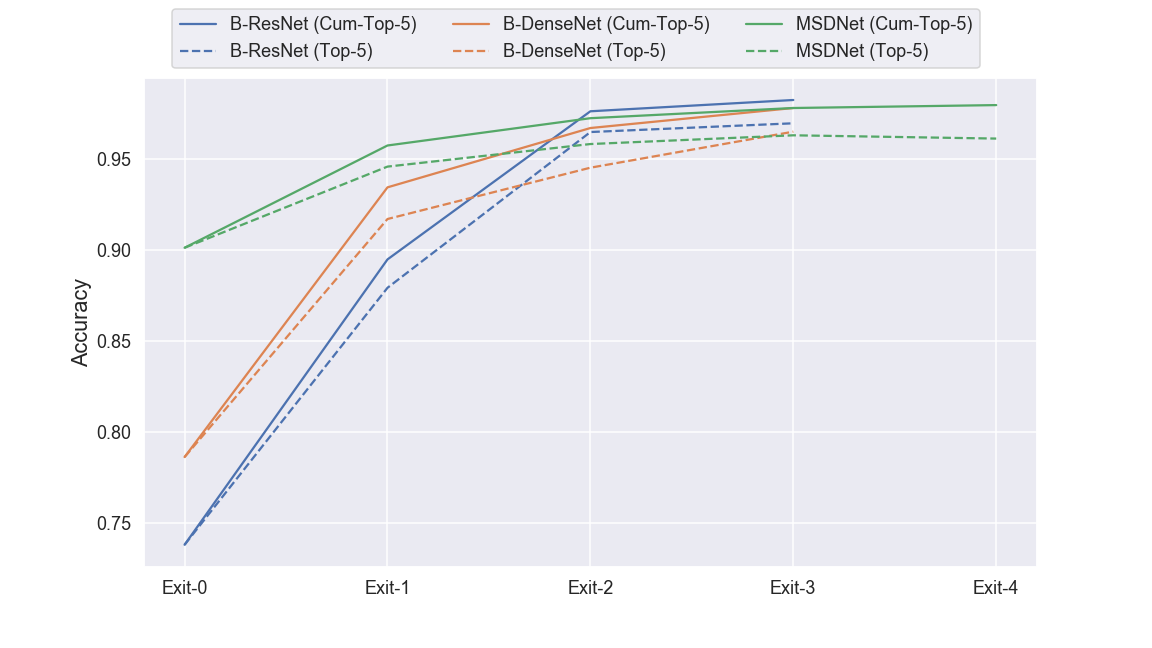
\includegraphics[width=.8\linewidth]{figures/edge/top5cumulative}
	\caption[Top-5 Cumulative]{Model Cumulative Top-5 Accuracy}
	\label{fig:top-5-cumulative}
\end{figure}

From the figure we can tell, that having multiple predictions does indeed improve the cumulative top-5. This means, there is a better chance of the correct label being in the set of predictions, when using all available exit outputs. In the next section we apply the information combination functions to data obtained from running the early exit model and collecting the output scores. 

In figure \ref{fig:theoretical-info-combi} we use the defined methods to combine the prediction information from multiple exits, to improve the overall model accuracy. 

The figure shows the obtainable accuracy given the number of exit predictions received. The brown line \textit{optimum-top5} show the maximum achievable accuracy, if we were able to cherry pick the right class among the cumulative top-5 predictions. The purple line, \textit{optimum-top1}, is the achievable accuracy, if we were always able to cherry pick the correct class among the cumulative top-1 predictions. 

Only the \gls{msdnet} shows a small improvement when adding predictions score exclusively, when all predictions are available. When predictions from all exits is not available, none of the propose combination methods are able to improve the accuracy.

The score margin produces the worst results. Thus, having a big difference between the two highest scoring classes is not equivalent with being correct. Using the confidence max achieves close to the same performance as using latest for \gls{bresnet} and \gls{bdensenet}. The conclusion is, combining the information using these simple methods, is not able to improve the accuracy of the model. In \cite{kaya_shallow-deep_nodate} they do not operate with a time constraint and always have all predictions. Our goal is to improve the accuracy, when all predictions are not available, as we cannot be sure to have received all predictions within the time frame.  Our results show, that simply using the latest received predictions, is the best overall choice for these early exit models. Henceforth we use the latest prediction, as this method gives the best results in general.  

\begin{figure}
	\captionsetup[subfigure]{justification=centering,farskip=1pt,captionskip=1pt}
	\centering
	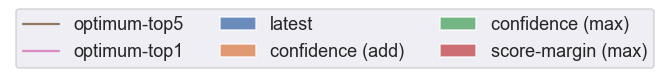
\includegraphics[width=.7\linewidth, keepaspectratio]{figures/edge/theoretical_score_combination_legend}
	\subfloat[B-ResNet]{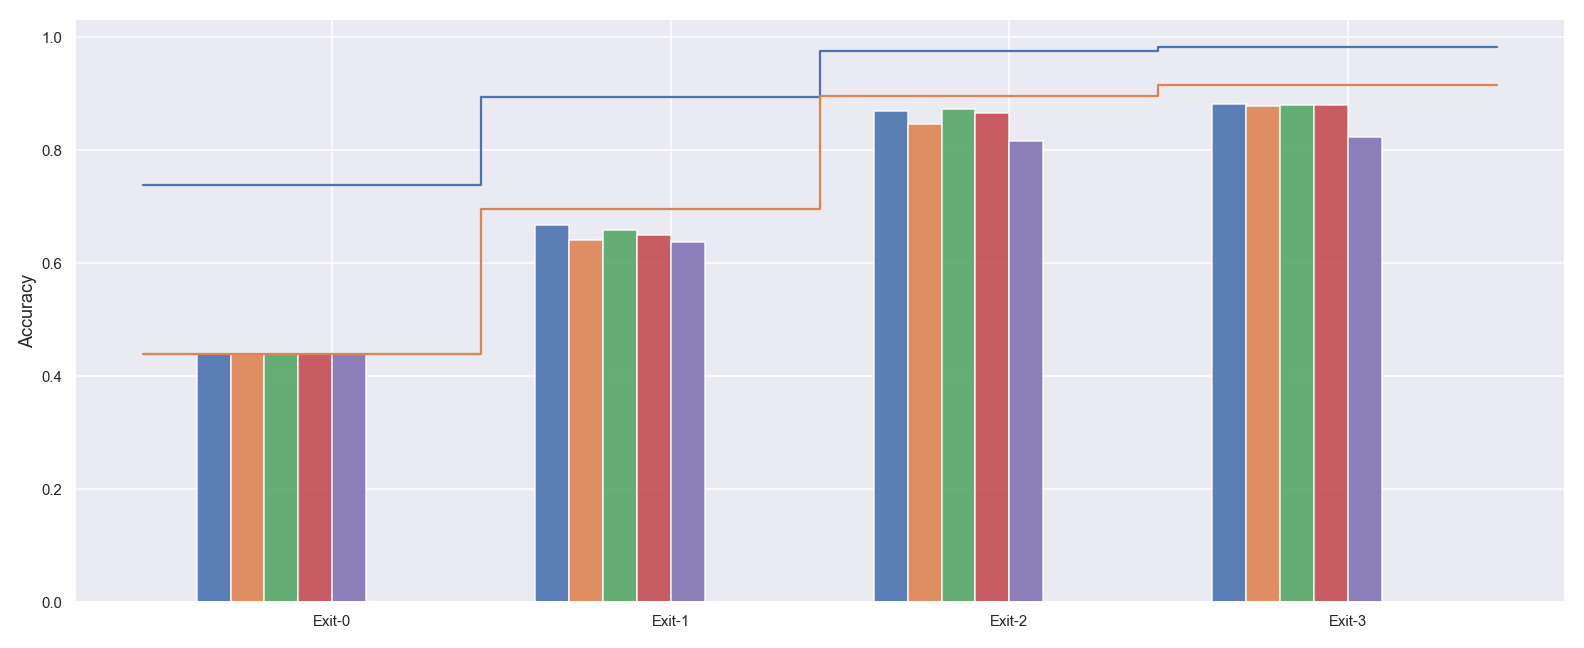
\includegraphics[height=.22\textheight, keepaspectratio]{figures/edge/b-resnet_theoretical_score_combinations}}
	\hfill
	\subfloat[B-DenseNet]{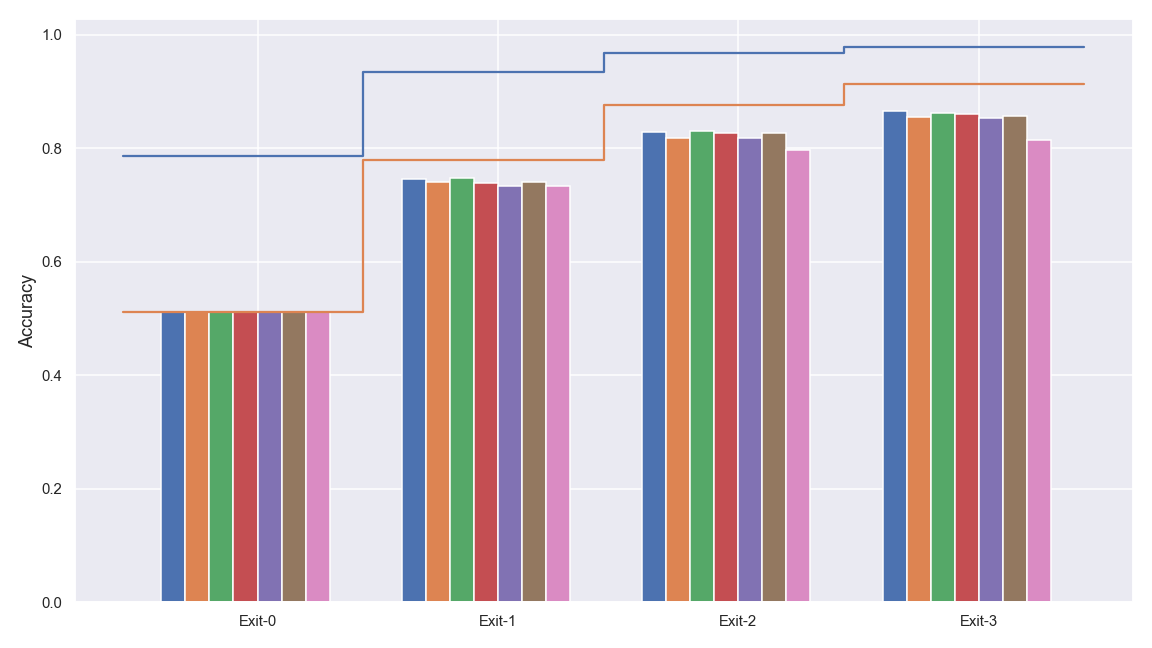
\includegraphics[height=.22\textheight, keepaspectratio]{figures/edge/b-densenet_theoretical_score_combinations}}
	\hfill
	\subfloat[MSDNet]{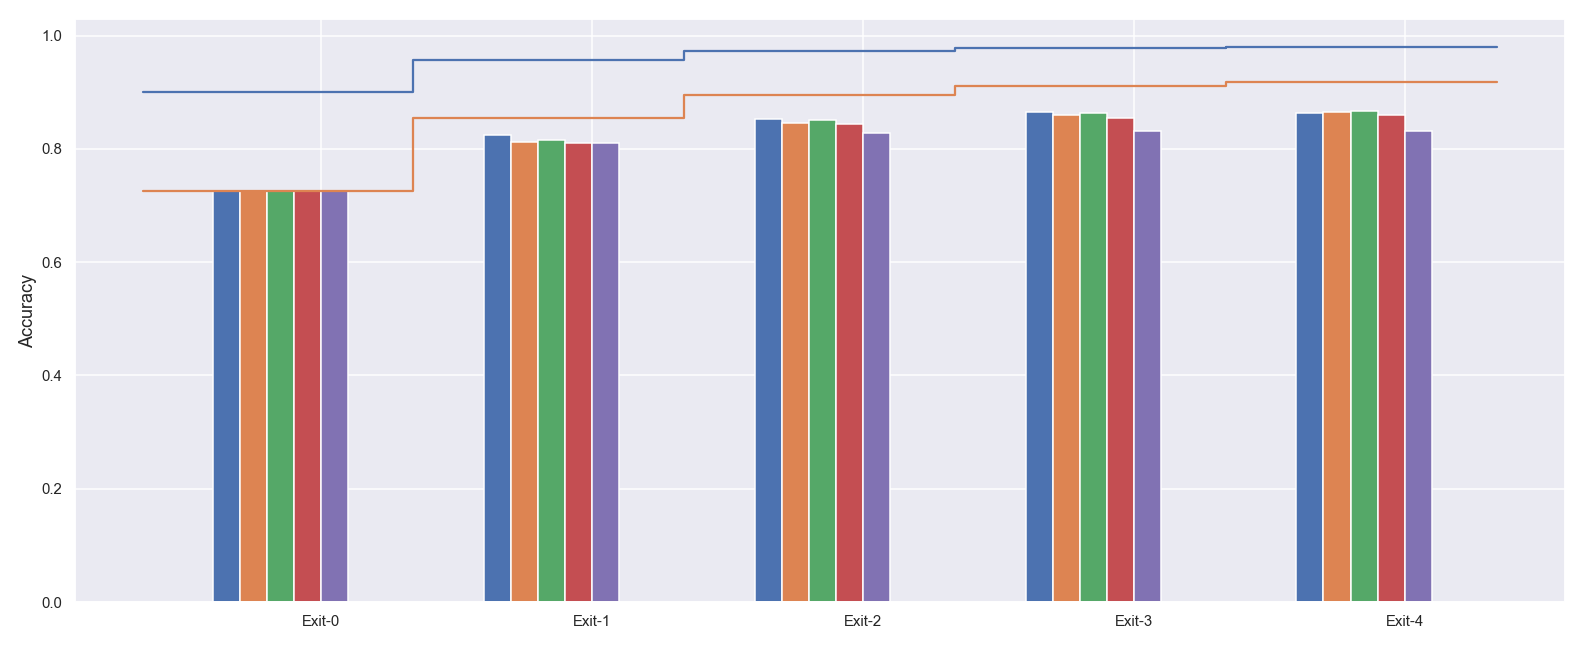
\includegraphics[height=.22\textheight, keepaspectratio]{figures/edge/msdnet_theoretical_score_combinations}}
	\caption[Combination Function with $ n $ Available Exits]{Combination Function with $ n $ Available Exits}
	\label{fig:theoretical-info-combi}
\end{figure}

We discuss the results using the combination functions in section \ref{sec:edge-summary}. 

\subsection{Edge Offloading: \gls{aee} vs Conventional Offloading}

We setup our system using NUC as end device and both \gls{jetson} and \gls{gpu-ws}. We set different delay thresholds and plot the achievable reliability using the prediction from the latest exit, see figure \ref{fig:practical-offloading}. Comparing with local execution in figure \ref{fig:delay-threshold}, the reliability deviates more from the added communication uncertainty, which makes the steps to next exit less sharp. It is clear from the figure, that no model, is always the best model at all delay threshold. From the figure, we can select the proper model given the delay threshold, by always selecting the model achieving the highest reliability.
\begin{figure}
	\captionsetup[subfigure]{justification=centering,farskip=1pt,captionskip=1pt}
	\centering
	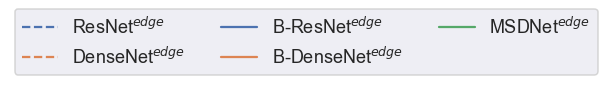
\includegraphics[width=.5\linewidth]{figures/edge/offloading_legend}
	\subfloat[\gls{jetson}]{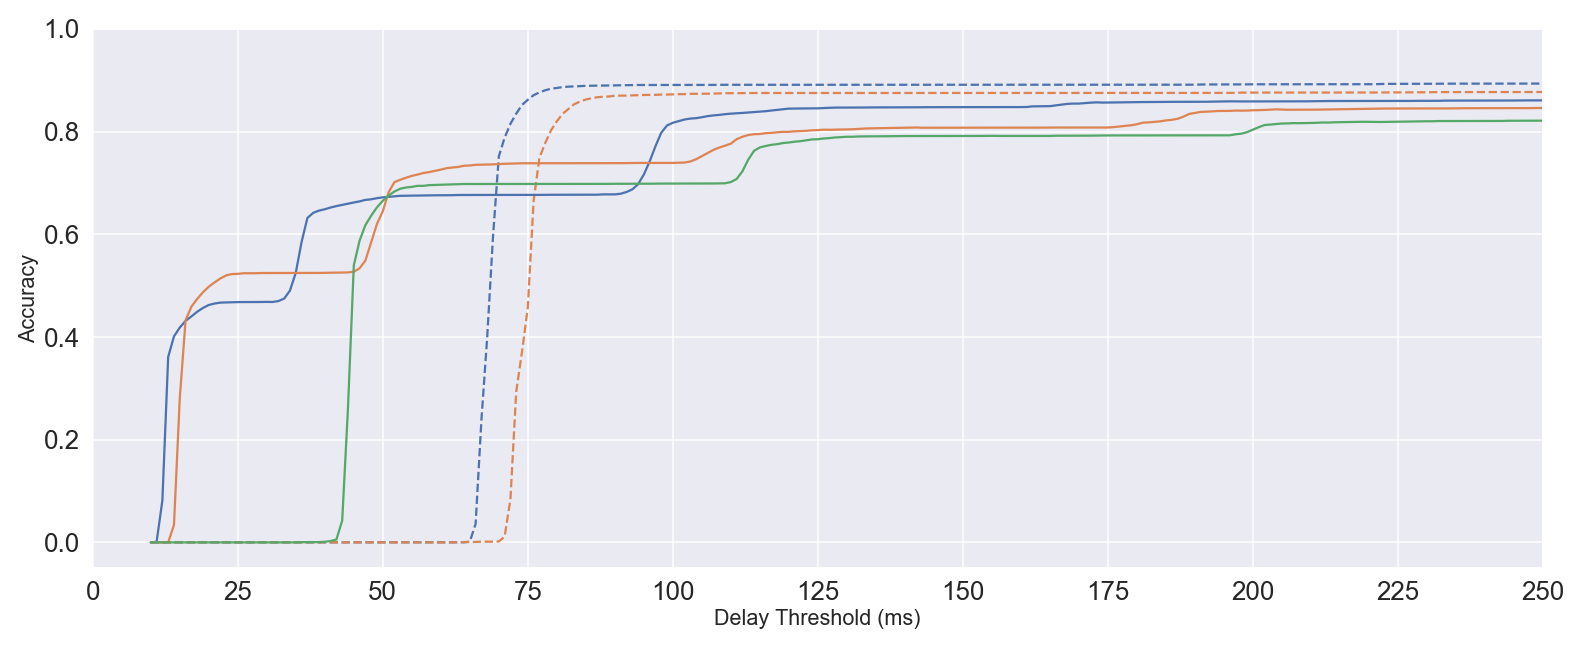
\includegraphics[width=.8\linewidth]{figures/edge/jetson_offloading}}
	\hfill
	\subfloat[\gls{gpu-ws}]{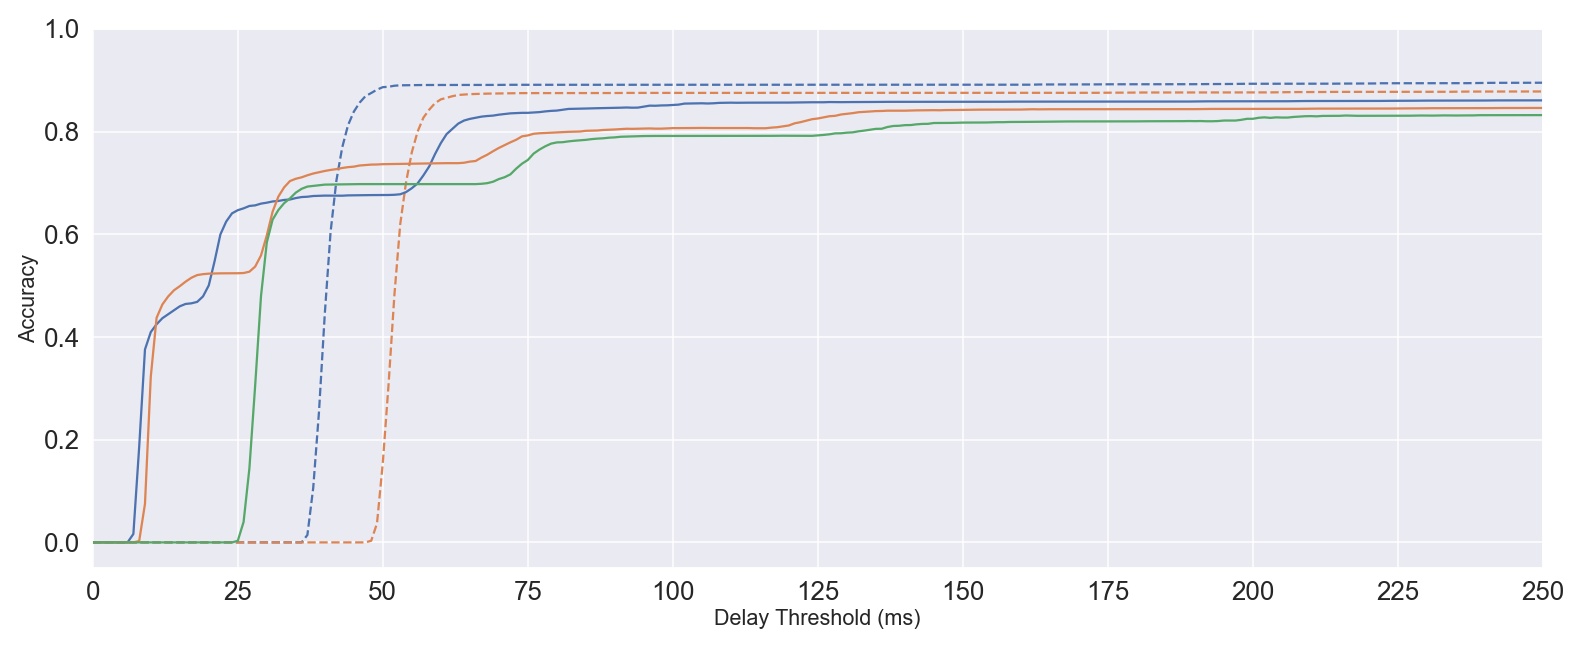
\includegraphics[width=.8\linewidth]{figures/edge/gpu_offloading}}
%	\subfloat[Local Jetson TX2]{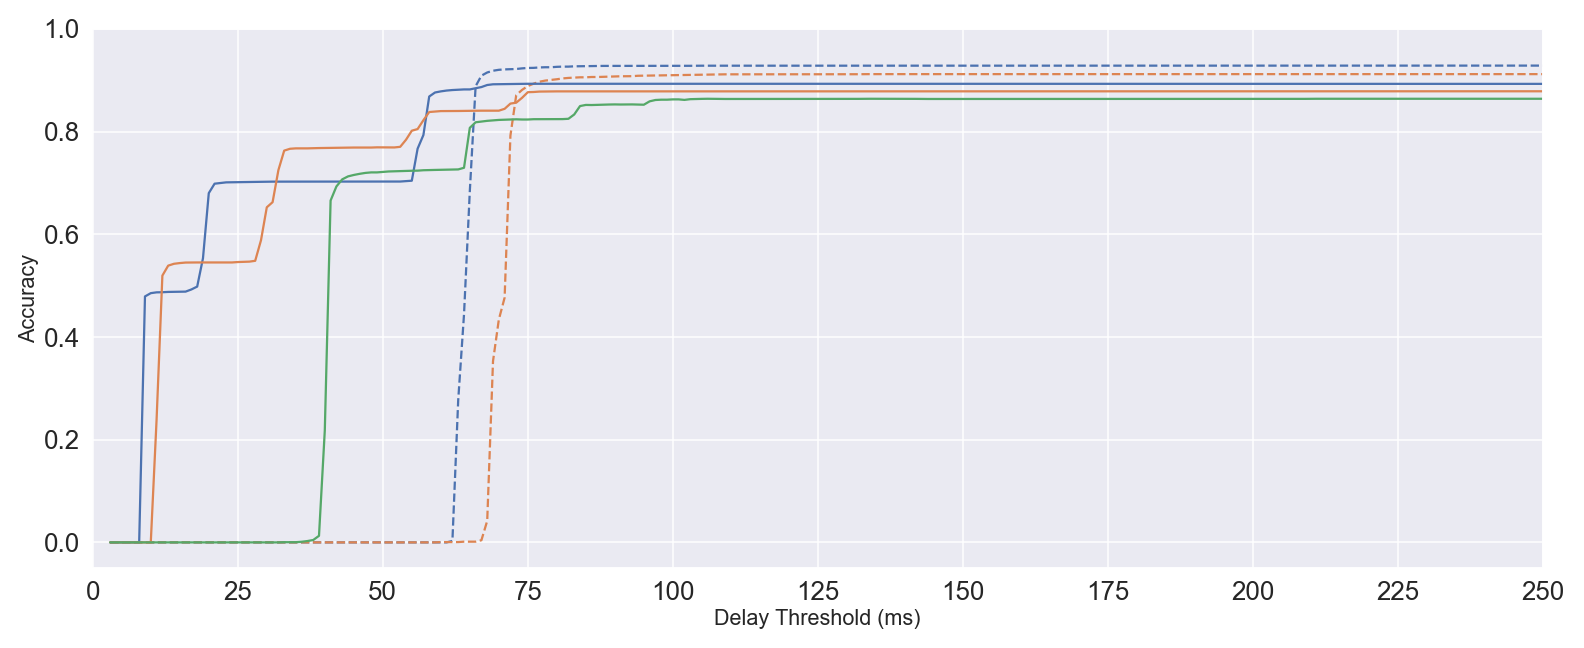
\includegraphics[width=\linewidth]{figures/delay_plots/jetson__delay_threshold}}
	\caption[Offloading NUC to Jetson]{Offloading NUC to Jetson}
	\label{fig:practical-offloading}
\end{figure}

The mean, standard deviation, minimum- and maximum value for the communication time is given in table \ref{tbl:time-offloading}. The mean of the added communication was 25 ms with a standard deviation of 110.93 ms, which clearly exemplifies the instability of communication delays. In worst case it takes almost 1 s to send an image.

\begin{longtabu}{>{\bfseries}X[2]|X|X|X|X}
	\caption[Communication Statistics]{Communication Statistics} \label{tbl:time-offloading} \\
	\toprule
	\rowfont{\bfseries} & Mean (ms) & Std. (ms) & Min (ms) & Max (ms) \tabularnewline
	\bottomrule
	\endfirsthead
	\multicolumn{3}{@{}l}{\textbf{\textcolor{black}{Table \ref{tbl:time-offloading}:}} continued}\\
	\toprule
	\rowfont{\bfseries} & Mean (ms) & Std. (ms) & Min (ms) & Max (ms) \tabularnewline
	\bottomrule
	\endhead % all the lines above this will be repeated on every page
	\bottomrule
	\multicolumn{3}{@{}l}{continued \ldots}\\
	\endfoot
	\hline
	\endlastfoot
	Communication time	& 25.68	& 110.93 & 2.35 & 962.76  \tabularnewline						
	\bottomrule
\end{longtabu}

We setup a test, where we sent the images from client to server. We logged the network traffic and analysed the number retransmission using \gls{wireshark} \cite{noauthor_wireshark_nodate}. Figure \ref{fig:tcp-overhead} shows the impact of \gls{tcp} retransmissions on the transmission delay. 

\begin{figure}
	\centering
	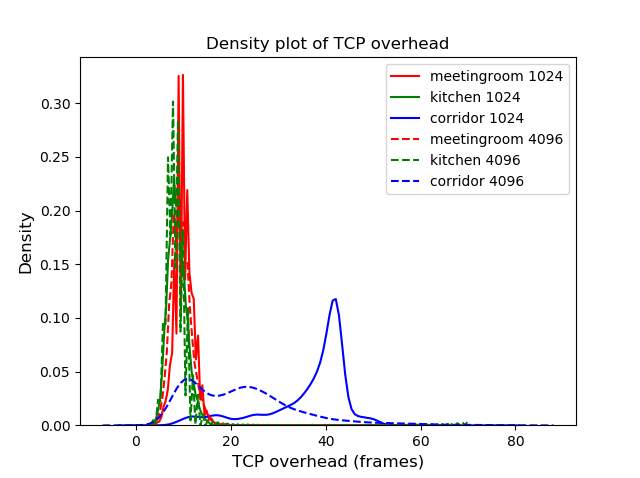
\includegraphics[width=.75\linewidth]{figures/tcp/tcpoverhead}
	\caption[TCP retransmission overhead]{TCP retransmission overhead}
	\label{fig:tcp-overhead}
\end{figure}

We repeated the test in three different scenarios (meetingroom, kitchen, and corridor). For the scenarios the end-device is moved further away from the server. The distance reduces the quality of the communication link. In poor communication environment \gls{tcp} can be expected to have a high overhead caused by increasing retransmissions, thus having a negative impact on the overall delay.  

\subsection{On-Device vs. Edge Offloading}

We have conducted experiments with using both \gls{jetson} and \gls{gpu-ws} as edge servers and \gls{nuc} as end device. We compare edge offloading the different models across the two edge platforms and with local inference on the \gls{nuc}. In figure \ref{fig:resnet-offloading-vs-local} we compare the \gls{resnet} based models. In figure \ref{fig:densenet-offloading-vs-local} the \gls{densenet} based models and lastly in figure \ref{fig:msdnet-offloading-vs-local} the \gls{msdnet} model.

\begin{figure}
	\captionsetup[subfigure]{justification=centering, farskip=0pt,captionskip=0pt}
	\centering
	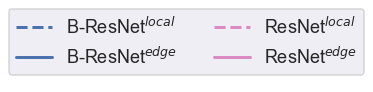
\includegraphics[width=.3\linewidth]{figures/edge/gpu_b-resnet_offloading_vs_local_legend}
	\hfill
	\subfloat[\gls{jetson} as Edge\label{fig:resnet-offloading-vs-local-jetson}]{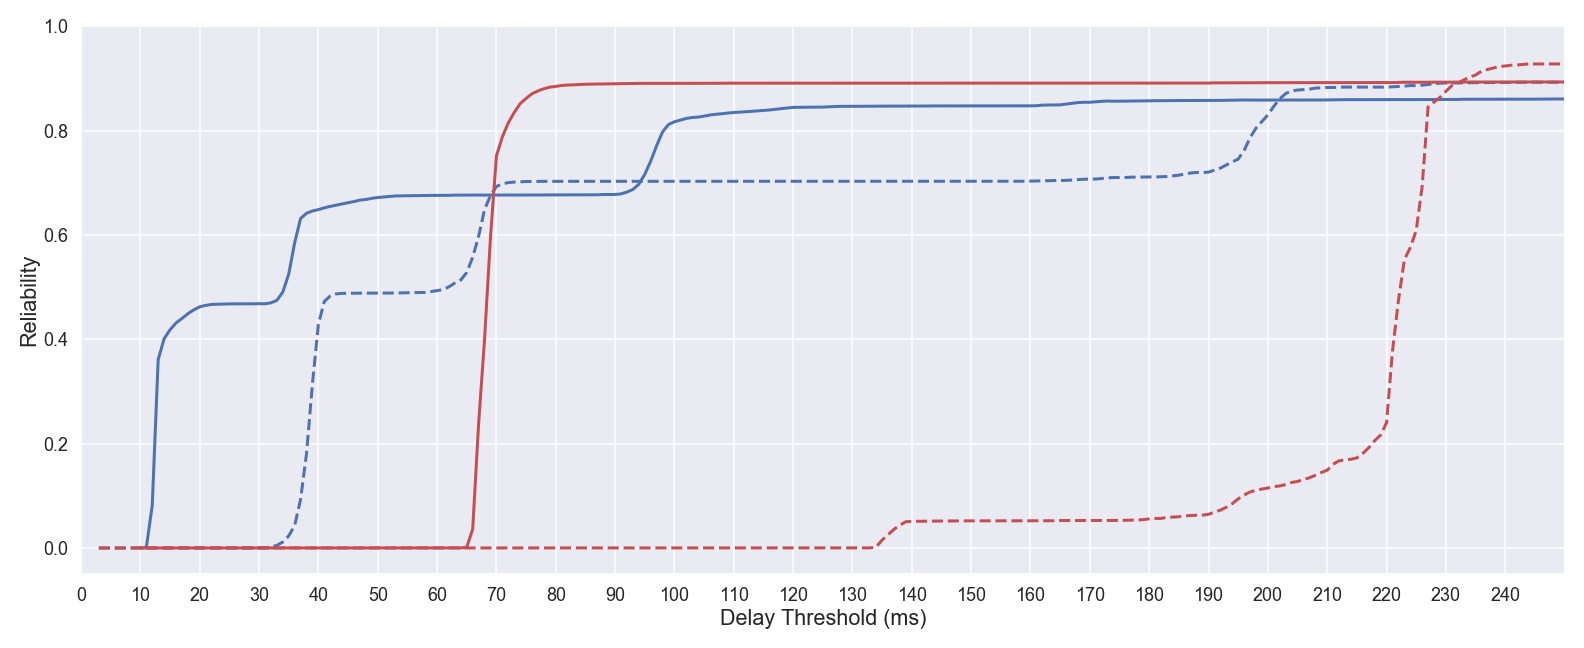
\includegraphics[width=\textwidth,height=.22\textheight,keepaspectratio]{figures/edge/jetson_b-resnet_offloading_vs_local}}
	\hfill
	\subfloat[\gls{gpu-ws} as Edge\label{fig:resnet-offloading-vs-local-gpu}]{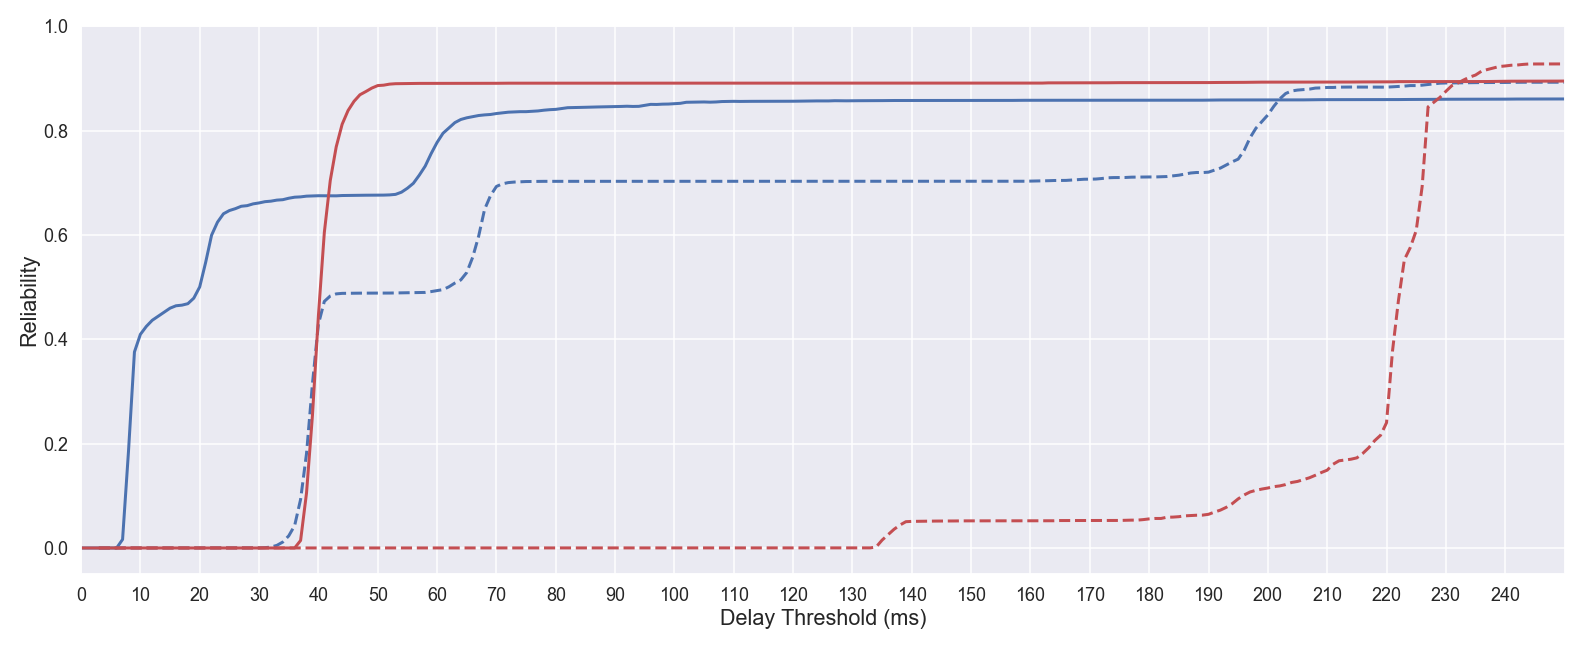
\includegraphics[width=\textwidth,height=.22\textheight,keepaspectratio]{figures/edge/gpu_b-resnet_offloading_vs_local}}
	\caption[Offloading comparison of residual networks]{Offloading comparison of residual networks}
	\label{fig:resnet-offloading-vs-local}
\end{figure}

From figure \ref{fig:resnet-offloading-vs-local} we can see, how the \gls{aee} scheme for edge offloading is able to improve the reliability under stringent delay requirement using either platform as edge server instead of local inference. We can also see, that it improve the reliability compared to using a conventional model again under stringent requirements. When offloading the conventional model, it starts to outperform the early exit model, if we allow 80 ms runtime using the Jetson TX2 or 50ms runtime using the GPU Workstation. Local inference would be the best option if the application can tolerate 250 ms delay, however, the time critical IoT applications requires much shorter delay threshold. The reason why local execution can obtain a higher reliability, is due to deadline violations caused by large variations in communication time. If we extend the x-axis to above 1 s, we would be able to see that the gap has been closed. 

\begin{figure}
	\captionsetup[subfigure]{justification=centering, farskip=0pt,captionskip=0pt}
	\centering
	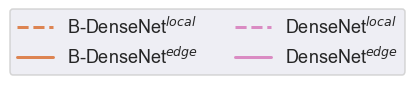
\includegraphics[width=.3\linewidth]{figures/edge/gpu_b-densenet_offloading_vs_local_legend}
	\hfill
	\subfloat[\gls{jetson} as Edge\label{fig:densenet-offloading-vs-local-jetson}]{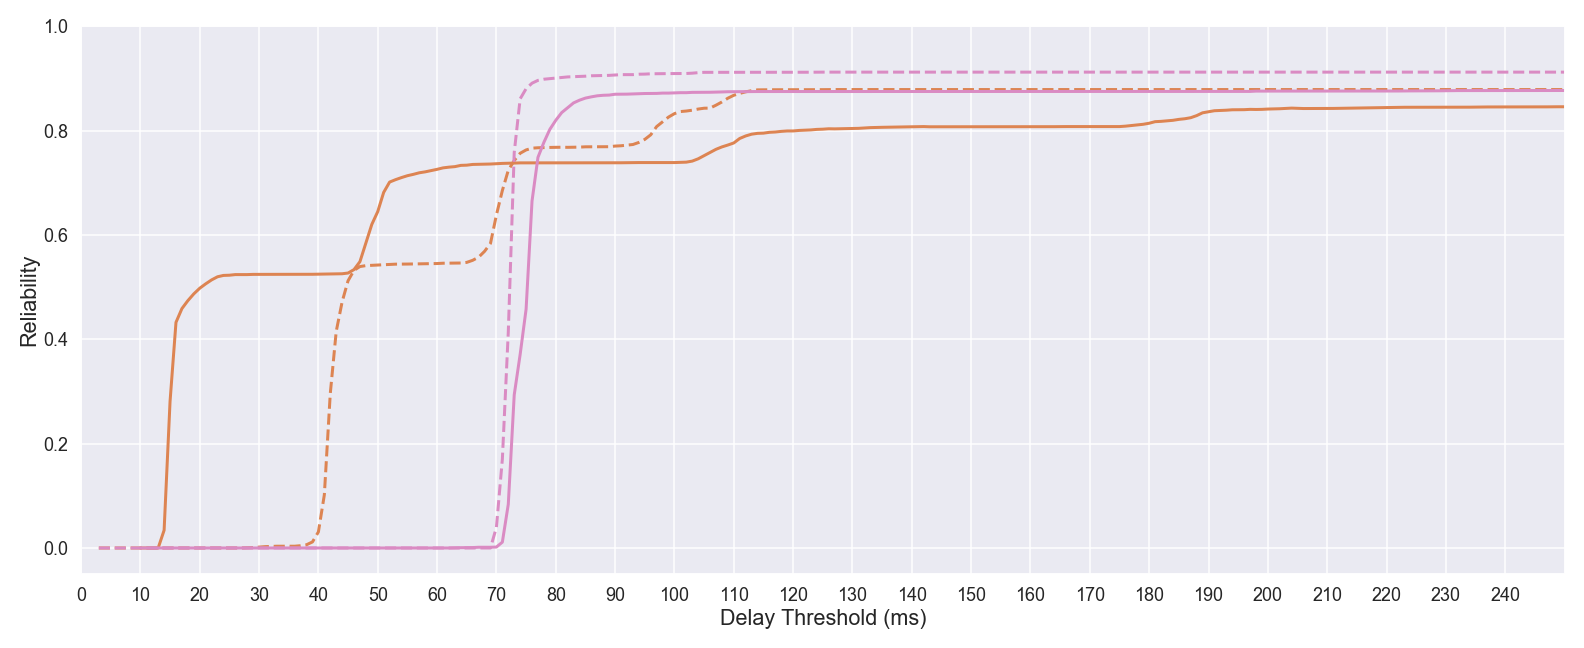
\includegraphics[width=\textwidth,height=.22\textheight,keepaspectratio]{figures/edge/jetson_b-densenet_offloading_vs_local}}
	\hfill
	\subfloat[GPU Workstation as Edge\label{fig:densenet-offloading-vs-local-gpu}]{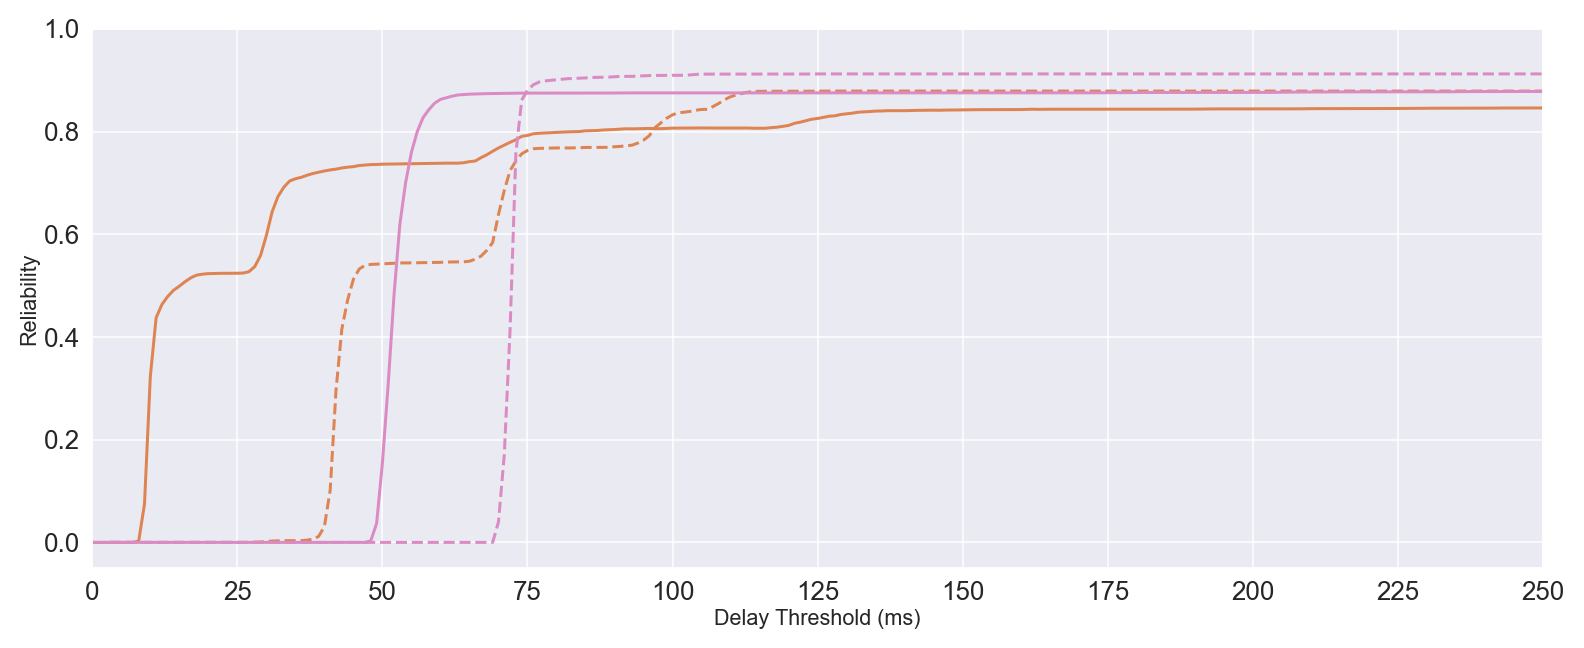
\includegraphics[width=\textwidth,height=.22\textheight,keepaspectratio]{figures/edge/gpu_b-densenet_offloading_vs_local}}
	\caption[Offloading comparison of densely connected networks]{Offloading comparison of densely connected networks}
	\label{fig:densenet-offloading-vs-local}
\end{figure}

The \gls{densenet} tells a somewhat different story. We are still able to improve reliability remarkably under stringent delay requirements using \gls{aee}, compared to offloading a conventional model or local inference. However, when reaching 70-80 ms on \gls{jetson} all other schemes, local inference B-\gls{densenet} or \gls{densenet} and also offloading \gls{densenet}, starts to outperform offloaded \gls{aee}. Local inference of the conventional model is even faster than offloading to \gls{jetson}. The performance difference between the \gls{jetson} and \gls{nuc} is not big enough for the \gls{densenet} based model, this we can tell from looking at \gls{gpu-ws}, where offloading the conventional model is performing better under 75 ms. 

\begin{figure}
	\captionsetup[subfigure]{justification=centering, farskip=0pt,captionskip=0pt}
	\centering
	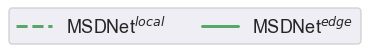
\includegraphics[width=.3\linewidth]{figures/edge/gpu_msdnet_offloading_vs_local_legend}
	\hfill
	\subfloat[\gls{jetson} as Edge]{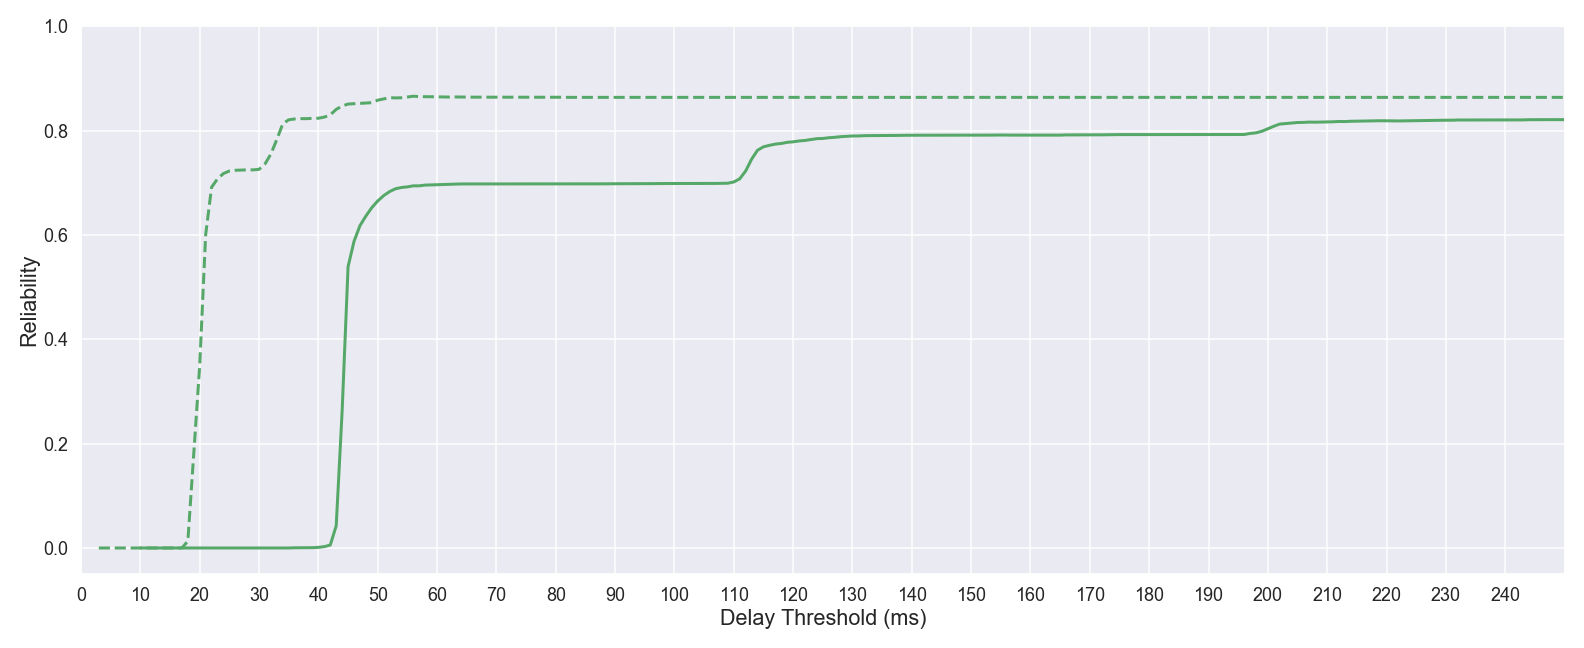
\includegraphics[width=\textwidth,height=.22\textheight,keepaspectratio]{figures/edge/jetson_msdnet_offloading_vs_local}}
	\hfill
	\subfloat[\gls{gpu-ws} as Edge]{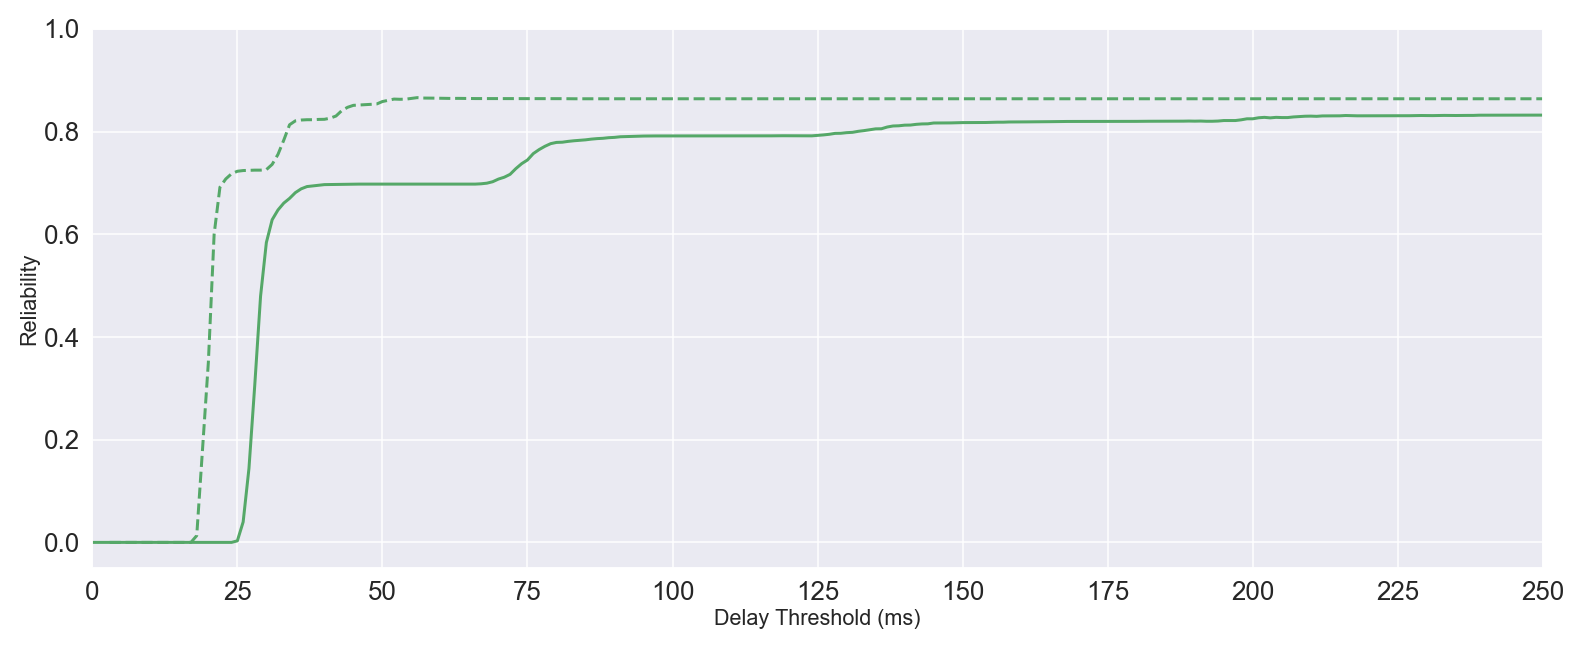
\includegraphics[width=\textwidth,height=.22\textheight,keepaspectratio]{figures/edge/gpu_msdnet_offloading_vs_local}}
	\caption[Offloading comparison of multi-scale dense networks]{Offloading comparison of multi-scale dense networks}
	\label{fig:msdnet-offloading-vs-local}
\end{figure}

\gls{msdnet} tells a completely different story. Local inference is always able to achieve higher reliability irregardless of offloading to \gls{jetson} or \gls{gpu-ws}. 

Offloading \gls{aee} to the edge improves system reliability in general compared to on-device \gls{aee} inference. Especially, \gls{aee} using \gls{bresnet} at the edge outperforms local inference of conventional \gls{resnet}. The improvement is most significant, when using the \gls{gpu-ws} which is a significantly more powerful machine compared to the \gls{jetson}. For the \gls{msdnet} our offloading solution was uncompetitive with local execution. The NUC is a very powerful end-device with a low power Intel i7 \gls{cpu}. In most scenarios in real-life end-device are more likely to be equipped with low-end ARM processors or even smaller processing units, which will degrade the inference time of any of the models. In \cite{zheng_apache/incubator-tvm_nodate}, they report average runtime of 726.0 ms of \gls{resnet}50 on Raspberry Pi, i.e. such low-end devices infeasible for real-time processing. Other end devices may not even be able to run any of the models locally. Given these results, the edge servers may not necessarily need to be equipped with powerful \gls{gpu}s, as the NUC is able to achieve such high performance running the \gls{msdnet}. These results clearly illustrates the complexity of offloading the inference task, as we were not able to find a single model, that provided the best reliability for all delay thresholds.

\section{Summary} \label{sec:edge-summary}

We investigated the overthinking phenomena and discovered some samples are correctly classified by an early exit, which a later exit wrongly classifies. In \cite{kaya_shallow-deep_nodate}, they show marginal improvements using the highest scoring prediction from all exits. Unfortunately, we did not achieve the same improvement using the confidence max. \gls{bresnet}'s and \gls{bdensenet}'s early exits have a rather low accuracy compared with its later exits, therefore introduces more uncertainty when combining the scores. The \gls{msdnet} on the other hand have decent accuracy at all exits, thus we were able to improve the accuracy when having all predictions available, when using the confidence sum function.

The improvement is most signifiant  Compared to local inference of early exit models we improve the reliability with the \gls{gpu-ws} as edge, however using the \gls{jetson} the \gls{bdensenet} is in fact providing a more reliable service locally, yet offloading to a stronger server, i.e. \gls{gpu-ws} show improvements.

Using \gls{aee} by offloading to the edge, service is enabled at stringent delay thresholds not possible, when offloading conventional models for edge inference. The scheme successfully improves the reliability below 75 ms for the \gls{jetson}, and below 50 ms for the \gls{gpu-ws} using \gls{bresnet} and \gls{bdensenet}. Offloading the different models show overlapping reliability of the \gls{bresnet} and \gls{bdensenet}, hence it depends on the delay threshold which model to select. 

In \gls{ddnn} \cite{teerapittayanon_distributed_2017}, a \gls{dnn} is used to fuse the output from early exits to combine the information. Running an additional \gls{dnn} for sensor fusion at the edge or on-device will cause additional delay, and take time away from running \gls{aee}. In \gls{ddnn} fused features come from a number of upstream devices, with exits at the same level. In our case we have predictions from different levels in the models. It will require future research to investigate, if improvement can be found fusing predictions from exits at different levels. Furthermore it will require an investigation of fusing data with different dimensions using \gls{dnn}s. 

The impact of communication uncertainties is shown in figures \ref{fig:resnet-offloading-vs-local}, \ref{fig:densenet-offloading-vs-local} and \ref{fig:msdnet-offloading-vs-local}. Compared to local execution, the steps in reliability have been smoothed out when time allows to reach a new exit, as the uncertainties of communication time, causes deadline violations and result in lost predictions. Our evaluation of \gls{tcp} at increasing distance indicates, that using \gls{tcp} leads to a large overhead in retransmission, resulting in additional delay. The communication latency could possibly be reduced, if the WiFi communication did not go through an access point. Instead the connection could be establish ad-hoc using WiFi Direct \cite{noauthor_wi-fi_nodate}. Or we could change the \gls{tcp} transport layer to \gls{udp}. \gls{tcp} was used for reliable transport to send a single jpeg image for processing, as jpeg is a lossless compression technique. Using \gls{udp} could cause loosing packets, which would impact the reconstruction of images server-side to be faulty and result in incorrectly classification, thus reducing the reliability. \gls{tcp} is not designed for video streaming applications, as retransmission of unacknowledged packet increase the communication delay. As shown in figure \ref{fig:tcp-overhead}, \gls{tcp} introduces a large overhead of retransmission, when networking conditions are poor. For video streaming \gls{udp} is more widely used. \gls{udp} is a more unreliable protocol, which is applicable in scenarios where some packet loss can be tolerated. The \gls{dnn}s may not be susceptible to small packet losses. In fact, the \gls{dnn}s have been trained with noise injection where pixels are randomly lost, see figure \ref{fig:augmentation}. For future research streaming jpeg compressed images over \gls{udp}, as in \cite{liu_maximizing_2019} would be interesting to investigate in order to reduce the communication latency. We did not pursue reducing the communication time, as our focus is not to obtain the best possible communication latency in this experimental setup, but rather show that \gls{aee} can reliably enable service at lower delays. 

Our inference scheme \gls{aee} is applicable for collaborative inference on device and edge, as in \cite{leroux_cascading_2017,teerapittayanon_distributed_2017}. Collaborative inference can be used to reduce the likelihood of missed predictions when experiencing sporadic communication delays. The on-device inference is only dependent on computation time for the local exits and removes the uncertainties from communicating with the edge server. However, the computing resources of the local device is typically significantly lower than the server's, which increases the delay and thereby reduces the chance of reaching a prediction from a later exit on the server due to time constraints. We investigated partitioning after the first exit, but encountered increased transmission delays, as the size of the intermediate features is remarkably larger than the compressed image's. We also experienced longer compute times locally for the first exit, which is more time consuming on the smaller device than on edge server for most models. The early layers of the \gls{dnn}s is typically also the most demanding, which leads even worse inference time locally. Thus, using collaborative inference degrades the reliability, when no feature compression or \gls{bottlenet} modules is used to reduce transmission time is used. Introducing feature compression would additionally require compression-aware retraining, as stated in \cite{choi_near-lossless_2018,choi_near-lossless_2018,eshratifar_bottlenet:_2019}  to avoid experiencing a high cost in accuracy. Further experimenting with this idea was considered out of scope for this project. Figure \ref{fig:resnet-offloading-vs-local} and \ref{fig:densenet-offloading-vs-local}, show the local inference time of the first exit of \gls{bresnet} and \gls{bdensenet}, is always outperformed by the edge servers. Therefore, offloading the entire task to not waste idle time a faster server.

An alternative solutions to handle the lost prediction dilemma, is a parallel execution of a shallower local \gls{dnn} and a deep remote \gls{dnn} i.e. a parallel Big/Little setup. The end device offloads the compressed image to edge server and in parallel process a smaller and less accurate \gls{dnn} locally. The upside is, that the application can always use the locally obtained prediction or choose to discard it, as more accurate prediction arrives from edge. Further if a good combination function is found, it can use the information to choose the best prediction. If on-device inference is not an option, then the offloading \gls{aee} is the better option.

We have not considered real-time processing a stream of video frames, but only single image classification. Comparing our inference scheme with Edgent, where an upfront selection of exit is done to handle the accuracy-latency trade-off. Edgent tries to utilize available time for the frame without postponing the next one. The selection of exit is based on regression models of inference time and a current state of bandwidth.  We argue, that the potential of early exiting is not fully utilizes by upfront sub-model selection. Upfront selection of exit is prone to loosing predictions caused by unexpected communication delays. If a timeout happens when exit 3 is selected, and the deadline is passed in block 3, no prediction will be provided.  In such cases our solutions will be more reliable, as the latency overhead of our additional exits classifier is negligible. Hence, when the deadline is violated, at least two predictions are available from exit 1 and exit 2. In other words, an early prediction is better than no predictions. Only in worst-case, where the first exit is unreachable neither \gls{aee} nor Edgent will suffice. 

If we encounter time-outs in between two exits the computation is wasted, which optimally could have been used to process the next frame, if the frame has been received. However, our solution fully utilizes the available time, if a next frame is not received. A future extension to our scheme is to let the server known the deadline and measured bandwidth, and have the server implement a decision based on elapsed time. If the server becomes aware, it cannot reach the next exit, it decides to terminate the inference process, and continue with the next received frame.

Edge/cloud offloading can potentially experience service outage. If an access point is no longer accessible, reconnection delays to a new or the same access point e.g. using WiFi can be expected to take up to 1 s \cite{pei_why_2017}. Which will inevitably lead to lost predictions, if no local inference is feasible. If local execution is feasible, we should switch to local execution of \gls{aee}, when experiences service outages, or switch to already proposed \gls{see} \cite{wang_see:_2019}. \gls{see} is a scheduling scheme to handle on-device inference of early exit \gls{dnn}s, if experiencing service outages to offloading services. 

